% !Mode:: "TeX:UTF-8"
\documentclass[newtxmath=true,newgeometry=two,capcenterlast=true,subcapcenterlast=true,openright=false,library=false,absupper=true,fontset=windowsnew,type=bachelor,campus=harbin]{hithesis}
% 此处选项中不要有空格
%%%%%%%%%%%%%%%%%%%%%%%%%%%%%%%%%%%%%%%%%%%%%%%%%%%%%%%%%%%%%%%%%%%%%%%%%%%%%%%%
% 必填选项
% type=doctor|master|bachelor
%%%%%%%%%%%%%%%%%%%%%%%%%%%%%%%%%%%%%%%%%%%%%%%%%%%%%%%%%%%%%%%%%%%%%%%%%%%%%%%%
% 选填选项(选填选项的缺省值已经尽可能满足了大多数需求,除非明确知道自己有什么
% 需求)
% campus=shenzhen|weihai|harbin
%   含义:校区选项,默认harbin
% glue=true|false
%   含义:由于我工规范中要求字体行距在一个闭区间内,这个选项为true表示tex自
%   动选择,为false表示区间内一个最接近版心要求行数的要求的默认值,缺省值为
%   false。
% tocfour=true|false
%   含义:是否添加第四级目录,只对本科文科个别要求四级目录有效,缺省值为
%   false
% fontset=siyuan|windowsnew|windowsold|mac|fandol
%   含义:注意这个选项视为了解决特殊问题而设置,比如用有些发行版本的linux排
%   版时可能(大多数发行版不会)会遇到的字体无法载入的问题,或者字体载入之
%   后出现无法复制的问题以及想要解决排版如 biang biang 面的 biang 这类中易
%   宋体无法识别的汉字的问题。没有特殊的需要不推荐使用这个选项。
%   
%   如果是安装了 windows 字体的 linux 系统,可以填写windowsnew(win vista
%   以后 的字体)或 windowsold(vista 以前)或者想用思源宋体并且是已经安装
%   了思源宋体的任何系统,填写siyuan选项。缺省值为空,自动识别系统并匹配字体
%   。模板版中给出的思源字体定义文件定义的思源字体的版本是Adobe版,其他字体
%   是windowsnew字体。(ps:Linux主流发行版ubuntu似乎要把思源字体作为默认字体)
%
%   如果是Mac系统,需要明确指定fontset=mac,由于各种各样的原因,多数情况是无法自
%   动识别mac系统字体,需要明确指定这个选项。注意,这时候使用的是mac系统中的宋
%   体,与windows中的宋体可能有点差别,虽然规范中没有明确规定使用那一种宋体,不
%   过按照窝工一贯的“规格严格,功夫到家”的风格,使用windows中的宋体肯定没毛病。
%   所以推荐Mac安装windows中的宋体。
%
%   fandol是一开源使用字体集,易于安装。这个选项放在这里是用来测试MacTeX/BasicTeX。
% tocblank=true|false
%   含义:目录中第一章之前,是否加一行空白。缺省值为true。
% chapterhang=true|false
%   含义:目录的章标题是否悬挂居中,规范中要求章标题少于15字,所以这个选项
%   有无没什么用,除了特殊需求。缺省值为true。
% fulltime=true|false
%   含义:是否全日制,缺省值为true。非全日制如同等学力等,要在cover中设置类
%   型,封面中不同格式
% subtitle=true|false
%   含义:论文题目是否含有副标题,缺省值为false,如果有要在cover中设置副标
%   题内容,封面中显示。
% newgeometry=one|two
%   含义:规范中的自相矛盾之处,版芯是否包含页眉页脚,旧方法是按照包含页眉
%   页脚来设置。该选项是多选选项,如果没有这个选项,缺省值是旧模板的版芯设
%   置方法,如果设置该选项one或two,分别对应两种页眉页码对应版芯线的相对位
%   置。第一种是严格按照规范要求,难看。第二种微调了页眉页码位置,好一点。
% debug=true|false
%   含义:是否显示版芯框和行号,用来调试。默认否。
% openright=true|false
%   含义:博士论文是否要求章节首页必须在奇数页,此选项不在规范要求中,按个
%   人喜好自行决定。 默认否。注意,窝工的默认情况是打印版博士论文要求右翻页
%   ,电子版要求非右翻页且无空白页。如果想DIY(或身不由己DIY)在什么地方右
%   翻页,将这个选项设置为false,然后在目标位置添加`\cleardoublepage`命令即
%   可。
% library=true|false
%   含义:是否为提交到图书馆的电子版。默认否。注意:如果设置成true,那么
%   openright选项将被强制转换为false。
% capcenterlast=true|false
%   含义:图题、表题最后一行是否居中对齐(我工规范要求居中,但不要求居中对
%   齐),此选项不在规范要求中,按个人喜好自行决定。默认否。
% subcapcenterlast=true|false
%   含义:子图图题最后一行是否居中对齐(我工规范要求居中,但不要求居中对齐
%   ),此选项不在规范要求中,按个人喜好自行决定。默认否。
% absupper=true|false
%   含义:中文目录中的英文摘要在中文目录中的大小写样式歧义,在规范中要求首
%   字母大写,在work样例中是全大写。该选项控制是否全大写。默认否。
% bsmainpagenumberline=true|false
%   含义:由于本科生论文官方模板的页码和页眉格式混乱,提供这个选项自定义设
%   置是否在正文中显示页码横线,默认否。
% bsfrontpagenumberline=true|false
%   含义:由于本科生论文官方模板的页码和页眉格式混乱,提供这个选项自定义设
%   置是否在前文中显示页码横线,默认否。
% bsheadrule=true|false
%   含义:由于本科生论文官方模板的页码和页眉格式混乱,提供这个选项自定义设
%   置是否显示页眉横线,默认显示。
% splitbibitem=true|false
%   含义:参考文献每一个条目内能不能断页,应广大刀客要求添加。默认否。
% newtxmath=true|false
%   含义:数学字体是否使用新罗马。默认是。
%%%%%%%%%%%%%%%%%%%%%%%%%%%%%%%%%%%%%%%%%%%%%%%%%%%%%%%%%%%%%%%%%%%%%%%%%%%%%%%%

\usepackage{hithesis}


\usepackage{algorithm} 
%\usepackage{algorithmic} 
\usepackage{multirow} 
\usepackage{algpseudocode}  
\usepackage{amsmath}
\usepackage{xcolor}  
\renewcommand{\algorithmicrequire}{\textbf{Input:}}  % Use Input in the format of Algorithm  
\renewcommand{\algorithmicensure}{\textbf{Output:}} % Use Output in the format of Algorithm  

\graphicspath{{figures/}}

\begin{document}

\frontmatter
% !Mode:: "TeX:UTF-8"

\hitsetup{
  %******************************
  % 注意:
  %   1. 配置里面不要出现空行
  %   2. 不需要的配置信息可以删除
  %******************************
  %
  %=====
  % 秘级
  %=====
  statesecrets={公开},
  natclassifiedindex={TM301.2},
  intclassifiedindex={62-5},
  %
  %=========
  % 中文信息
  %=========
  ctitleone={基于深度强化学习的},%本科生封面使用
  ctitletwo={异构系统频谱智能分配},%本科生封面使用
  ctitlecover={基于深度强化学习的异构系统\\频谱智能分配},%放在封面中使用,自由断行
  ctitle={基于深度强化学习的异构系统频谱智能分配},%放在原创性声明中使用
  %csubtitle={一条副标题}, %一般情况没有,可以注释掉
  cxueke={工学},
  csubject={通信工程},
  caffil={电子与信息工程学院},
  cauthor={陈鹏},
  csupervisor={高玉龙},
  %  cassosupervisor={某某某教授}, % 副指导老师
  %  ccosupervisor={某某某教授}, % 联合指导老师
  % 日期自动使用当前时间,若需指定按如下方式修改:
  cdate={2020年6月11日},
  cstudentid={1160500920},
  %cstudenttype={同等学力人员}, %非全日制教育申请学位者
  %(同等学力人员)、(工程硕士)、(工商管理硕士)、
  %(高级管理人员工商管理硕士)、(公共管理硕士)、(中职教师)、(高校教师)等
  %
  %
  %=========
  % 英文信息
  %=========
  etitle={Research on key technologies of partial porous externally pressurized gas bearing},
  esubtitle={This is the sub title},
  exueke={Engineering},
  esubject={Computer Science and Technology},
  eaffil={\emultiline[t]{School of Mechatronics Engineering \\ Mechatronics Engineering}},
  eauthor={Yu Dongmei},
  esupervisor={Professor XXX},
  eassosupervisor={XXX},
  % 日期自动生成,若需指定按如下方式修改:
  edate={December, 2017},
  estudenttype={Master of Art},
  %
  % 关键词用“英文逗号”分割
  ckeywords={分簇模型, 频谱分配, 深度强化学习, 长短期记忆网络},
  ekeywords={cluster model, spectrum allocation, DRL, LSTM},
}

\begin{cabstract}

随着未来空天地一体化通信框架的提出,各种系统的用户将共享频谱资源。这使得本就紧张的频谱资源变得更为珍贵,为此本文考虑异构系统中频谱的动态与智能分配问题,将其构建其为部分观测马尔可夫决策过程。在空天地一体化通信框架下,本文提出以用户为中心的分布式智能资源分配,提出分簇模型代替原有地面蜂窝网架构,让用户以自组织形式成为簇头或簇内用户并进行资源自主分配。簇头在考虑用户数量及用户移动性等因素后自主决策簇大小及资源提供总量,用户对这些资源进行申请,最终由簇头进行分配。将通信链路建立和资源分配流程细分为三个部分:簇头选择,信道分配,功率控制。在传统算法难以解决的前提下,使用深度强化学习解决该问题。以集中离线训练方式对当前可接入簇头状态进行预测,给出最优簇头选择方案,方案中用户通过相同网络构架DRQN选择信道,避免冲突,最后在簇头用户成功连接前提下进行功率方面调节。在保证用户通信体验同时提高频谱的利用效率,使整个网络吞吐量最大化。

本文在传统的强化学习(RL)的基础上融合深度神经网络,形成深度强化学习(DRL),提高智能体对输入数据为连续信息情况下的识别能力。加入长短期记忆网络(LSTM),提高智能体对连续历史信息的处理能力,使其可以依据既往信息对当前状态进行有效预测。通过强化学习独有的决策能力获取最优动作,以此得到问题近似最优解。通过借鉴已有方法将网络切分为状态网络和动作优势网络,并加入目标网络形成双网络架构来优化DRQN网络,使智能体在实现高效训练,快速收敛的基础上获得更稳定的收敛效果。

在具体仿真和验证过程中给出具体操作流程,依据问题的不同细节进行算法调整,并对仿真测试结果进行直观化展示以及分析,验证算法适用性以及对比传统算法优势,得到较为满意结果。初步形成一个完整,可行,有效的新型通信框架下的异构系统资源分配算法。并于最后对已完成工作进行总结评价,并为未来频谱资源高效利用提出创新性建议。

\end{cabstract}

\begin{eabstract}
   
   With the proposed future integrated communication framework for space, air and ground, users of various systems will share the scarce spectrum resources.We consider the problem of spectrum allocation in a dynamic heterogeneous system which is formulated as a partially observable Markov decision process. Under the frame of Space-air-ground integration network(SAGIN), we propose a new model of cluster to replace the cellular network which is user-centric distributed intelligent resource allocation. Users can self-organized to be cluster head or in-cluster users and they can autonomous allocation of resources.The communication link establishment and resource allocation process is subdivided into three parts: cluster head selection, channel allocation, and power control. We apply deep reinforcement learning to solve the problem. We train the agent at central unit in an offline manner to have the ability of predicting the current state of the cluster head. In addition, the agent can use the same network frame to choose a specific channel and get on power control. Therefore the spectrum utilization can be improved and maximize whole network throughput.
   
   We merge deep neural network(DL) with the reinforcement learning(RL), which come to deep reinforcement learning(DRL),it can settle high-dimensional input data. In addition, we add LSTM to predict the state according to the past information. By referring to existing methods, the network is divided into state network and action advantage network, and the target network is added to form a double network architecture to optimize the DRQN network, so that the agent can obtain more stable convergence effects on the basis of efficient training and rapid convergence. 

   In the specific simulation and verification process, the algorithm is adjusted and improved according to the different details of the problem, and the simulation test results are visually displayed and performance analysis. result. A complete, feasible, and effective new communication resource allocation algorithm for heterogeneous systems is initially formed. And at the end, it summarizes and evaluates the completed work, and puts forward innovative suggestions for the efficient use of spectrum resources in the future.
\end{eabstract}
 % 封面
\makecover
\begin{denotation}
\begin{table}[h]%此处最好是h
\caption{国际单位制中具有专门名称的导出单位}
\vspace{0.5em}\centering\wuhao
\begin{tabular}{cccc}
\toprule[1.5pt]
量的名称&单位名称&单位符号&其它表示实例\\
\midrule[1pt]
频率&赫[兹]&Hz&$s^_{-1}$\\
长度&米&m&m\\
时间&秒&s&s\\
功率;辐射通量&瓦[特]&W&W\\


\bottomrule[1.5pt]
\end{tabular}
\end{table}
\end{denotation}
%物理量名称表,符合规范为主,有要求添加
%\cleardoublepage  自定义在什么位置进行右翻页
\tableofcontents    % 中文目录
%\cleardoublepage  自定义在什么位置进行右翻页
%\tableofengcontents % 英文目录,硕本不要求

\mainmatter
%\linenumbers %debug 选项
%\layout %debug 选项
%\floatdiagram %debug 选项
%\begin{figure} %debug 选项
%\currentfloat %debug 选项
%\tryintextsep{\intextsep} %debug 选项
%\trytopfigrule{0.5pt} %debug 选项
%\trybotfigrule{1pt} %debug 选项
%\setlayoutscale{0.9} %debug 选项
%\floatdesign %debug 选项
%\caption{Float layout with rules}\label{fig:fludf} %debug 选项
%\end{figure} %debug 选项
%\include{body/regu}
%% !Mode:: "TeX:UTF-8"

\chapter{示例文档}[Example]

这是 \hithesis\ 的示例文档,基本上覆盖了模板中所有格式的设置。建议大家在使用模
板之前,除了阅读《\hithesis\:哈尔滨工业大学学位论文模板》\footnote{即
hithesis.pdf文件},本示例文档也最好能看一看。此示例文档尽量使用到所有的排版格式
,然而对于一些不在我工规范中规定的文档,理论上是由用户自由发挥,这里不给出样例
。需要另行载入的宏包和自定义命令在文件`hithesis.sty'中有示例,这里不列举。

\section{关于数字}[Number]

按《关于出版物上数字用法的试行规定》(1987年1月1日国家语言文字工作委员会等7个单位公布),除习惯用中文数字表示的以外,一般数字均用阿拉伯数字。
(1)公历的世纪、年代、年、月、日和时刻一律用阿拉伯数字,如20世纪,80年代,4时3刻等。年号要用四位数,如1989年,不能用89年。
(2)记数与计算(含正负整数、分数、小数、百分比、约数等)一律用阿拉伯数字,如3/4,4.5%,10个月,500多种等。
(3)一个数值的书写形式要照顾到上下文。不是出现在一组表示科学计量和具有统计意义数字中的一位数可以用汉字,如一个人,六条意见。星期几一律用汉字,如星期六。邻近两个数字并列连用,表示概数,应该用汉字数字,数字间不用顿号隔开,如三五天,七八十种,四十五六岁,一千七八百元等。
(4)数字作为词素构成定型的词、词组、惯用语、缩略语等应当使用汉字。如二倍体,三叶虫,第三世界,“七五”规划,相差十万八千里等。
(5)5位以上的数字,尾数零多的,可改写为以万、亿为单位的数。一般情况下不得以十、百、千、十万、百万、千万、十亿、百亿、千亿作为单位。如~\num{345000000}~公里可改写为3.45亿公里或~\num{34500}~万公里,但不能写为3亿~\num{4500}~万公里或3亿4千5百万公里。
(6)数字的书写不必每格一个数码,一般每两数码占一格,数字间分节不用分位号“,”,凡4位或4位以上的数都从个位起每3位数空半个数码(1/4汉字)。“\num{3000000}”,不要写成“3,000,000”,小数点后的数从小数点起向右按每三位一组分节。一个用阿拉伯数字书写的多位数不能从数字中间转行。
(7)数量的增加或减少要注意下列用词的概念:1)增加为(或增加到)过去的二倍,即过去为一,现在为二;2)增加(或增加了)二倍,即过去为一,现在为三;3)超额80%,即定额为100,现在为180;4)降低到80%,即过去为100,现在为80;5)降低(或降低了)80%,即原来为100,现在为20;6)为原数的1/4,即原数为4,现在为1,或原数为1,现在为0.25。
应特别注意在表达数字减小时,不宜用倍数,而应采用分数。如减少为原来的1/2,1/3等。


\section{索引示例}[Index]

为便于检索文中内容,可编制索引置于论文之后(根据需要决定是否设置)。索引以论文中
的专业词语为检索线索,指出其相关内容的所在页码。索引用中、英两种文字书写,中文在
前。\sindex[china]{qi!乔峰}\sindex[english]{Xu Zhu}\sindex[english]{Qiao Feng}
中文按各词汉语拼音第一个字母排序,英文按该词第一个英文字母排序。

\section{术语排版举例}[Glossaries and index]

术语的定义和使用可以结合索引,灵活使用。
例如,\gtssbp 是一种应用于狄利克雷过程抽样的算法。
下次出现将是另一种格式:\gtssbp 。
还可以切换单复数例如:\gscnas ,下次出现为:\gscnas 。
此处体现了\LaTeX\ 格式内容分离的优势。

\section{引用}[Cite]

\sindex[china]{du!段誉}引文标注遵照GB/T7714-2005,采用顺序编码制。正文中引用文献的标示应置于所引内容最后一个字的右上角,所引文献编号用阿拉伯数字置于方括号“[ ]”中,用小4号字体的上角标。要求:

(1)引用单篇文献时,如“二次铣削\cite{cnproceed}”。

(2)同一处引用多篇文献时,各篇文献的序号在方括号内全部列出,各序号间用“,”,如
遇连续序号,可标注讫序号。如,…形成了多种数学模型\cite{cnarticle,cnproceed}…
注意此处添加\cs{inlinecite}中文空格\inlinecite{cnarticle,cnproceed},可以在cfg文件中修改空格类型。

(3)多次引用同一文献时,在文献序号的“[ ]”后标注引文页码。如,…间质细胞CAMP含量
测定\cite[100-197]{cnarticle}…。…含量测定方法规定
\cite[92]{cnarticle}…。

(4)当提及的参考文献为文中直接说明时,则用小4号字与正文排齐,如“由文献\inlinecite{hithesis2017}可知”

\section{定理和定义等}[Theorem]
\begin{theorem}[\cite{cnproceed}]
宇宙大爆炸是一种爆炸。
\end{theorem}
\begin{definition}[(霍金)]
宇宙大爆炸是一种爆炸。
\end{definition}
\begin{assumption}
宇宙大爆炸是一种爆炸。
\end{assumption}
\begin{lemma}
宇宙大爆炸是一种爆炸。
\end{lemma}
\begin{corollary}
宇宙大爆炸是一种爆炸。
\end{corollary}
\begin{exercise}
宇宙大爆炸是一种爆炸。
\end{exercise}
\begin{problem}[(Albert Einstein)]
宇宙大爆炸是一种爆炸。
\end{problem}
\begin{remark}
宇宙大爆炸是一种爆炸。
\end{remark}
\begin{axiom}[(爱因斯坦)]
宇宙大爆炸是一种爆炸。
\end{axiom}
\begin{conjecture}
宇宙大爆炸是一种爆炸。
\end{conjecture}
\section{图片}[Pictures]
图应有自明性。插图应与文字紧密配合,文图相符,内容正确。选图要力求精练,插图、照
片应完整清晰。机械工程图:采用第一角投影法,严格按照GB4457~GB131-83《机械制图》
标准规定。数据流程图、程序流程图、系统流程图等按GB1526-89标准规定。电气图:图形
符号、文字符号等应符合附录3所列有关标准的规定。流程图:必须采用结构化程序并正确
运用流程框图。对无规定符号的图形应采用该行业的常用画法。坐标图的坐标线均用细实线
,粗细不得超过图中曲线;有数字标注的坐标图,必须注明坐标单位。照片图要求主题和主
要显示部分的轮廓鲜明,便于制版。如用放大或缩小的复制品,必须清晰,反差适中。照片
上应有表示目的物尺寸的标度。引用文献中的图时,除在正文文字中标注参考文献序号以外
,还必须在中、英文表题的右上角标注参考文献序号。

\subsection{博士毕业论文双语题注}[Doctoral picture example]
\begin{figure}[htpb]
\centering
\includegraphics[width = 0.4\textwidth]{golfer}
\bicaption[golfer1]{}{打高尔夫球球的人(博士论文双语题注)}{Fig.$\!$}{The person playing golf (Doctoral thesis)}
\end{figure}

每个图均应有图题(由图序和图名组成),图题不宜有标点符号,图名在图序之后空1个半
角字符排写。图序按章编排,如第1章第一个插图的图号为“图1-1”。图题置于图下,硕士论
文只用中文,博士论文用中、英两种文字,居中书写,中文在上,要求中文用宋体5号字,
英文用Times New Roman 5号字。有图注或其它说明时应置于图题之上。引用图应注明出处
,在图题右上角加引用文献号。图中若有分图时,分图题置于分图之下或图题之下,可以只
用中文书写,分图号用a)、b)等表示。图中各部分说明应采用中文(引用的外文图除外)或
数字符号,各项文字说明置于图题之上(有分图时,置于分图题之上)。图中文字用宋体、
Times New Roman字体,字号尽量采用5号字(当字数较多时可用小5号字,以清晰表达为原
则,但在一个插图内字号要统一)。同一图内使用文字应统一。图表中物理量、符号用斜体
。
\subsection{本硕论文题注}[Other picture example]
\begin{figure}[h]
\centering
\includegraphics[width = 0.4\textwidth]{golfer}
\caption{打高尔夫球的人,硕士论文要求只用汉语}
\end{figure}

\subsection{并排图和子图}[Abreast-picture and Sub-picture example]
\subsubsection{并排图}[Abreast-picture example]

使用并排图时,需要注意对齐方式。默认情况是中部对齐。这里给出中部对齐、顶部对齐
、图片底部对齐三种常见方式。其中,底部对齐方式有一个很巧妙的方式,将长度比较小
的图放在左面即可。

\begin{figure}[htbp]
\centering
\begin{minipage}{0.4\textwidth}
\centering
\includegraphics[width=\textwidth]{golfer}
\bicaption[golfer2]{}{打高尔夫球的人}{Fig.$\!$}{The person playing golf}
\end{minipage}
\centering
\begin{minipage}{0.4\textwidth}
\centering
\includegraphics[width=\textwidth]{golfer}
\bicaption[golfer3]{}{打高尔夫球的人。注意,这里默认居中}{Fig.$\!$}{The person playing golf. Please note that, it is vertically center aligned by default.}
\end{minipage}
\end{figure}

\begin{figure}[htbp]
\centering
\begin{minipage}[t]{0.4\textwidth}
\centering
\includegraphics[width=\textwidth]{golfer}
\bicaption[golfer5]{}{打高尔夫球的人}{Fig.$\!$}{The person playing golf}
\end{minipage}
\centering
\begin{minipage}[t]{0.4\textwidth}
\centering
\includegraphics[width=\textwidth]{golfer}
\bicaption[golfer8]{}{打高尔夫球的人。注意,此图是顶部对齐}{Fig.$\!$}{The person playing golf. Please note that, it is vertically top aligned.}
\end{minipage}
\end{figure}

\begin{figure}[htbp]
\centering
\begin{minipage}[t]{0.4\textwidth}
\centering
\includegraphics[width=\textwidth,height=\textwidth]{golfer}
\bicaption[golfer9]{}{打高尔夫球的人。注意,此图对齐方式是图片底部对齐}{Fig.$\!$}{The person playing golf. Please note that, it is vertically bottom aligned for figure.}
\end{minipage}
\centering
\begin{minipage}[t]{0.4\textwidth}
\centering
\includegraphics[width=\textwidth]{golfer}
\bicaption[golfer6]{}{打高尔夫球的人}{Fig.$\!$}{The person playing golf}
\end{minipage}
\end{figure}

\subsubsection{子图}[Sub-picture example]
注意:子图题注也可以只用中文。规范规定“分图题置于分图之下或图题之下”,但没有给出具体的格式要求。
没有要求的另外一个说法就是“无论什么格式都不对”。
所以只有在一个图中有标注“a),b)”,无法使用\cs{subfigure}的情况下,使用最后一个图例中的格式设置方法,否则不要使用。
为了应对“无论什么格式都不对”,这个子图图题使用“minipage”和“description”环境,宽度,对齐方式可以按照个人喜好自由设置,是否使用双语子图图题也可以自由设置。

\begin{figure}[!h]
\setlength{\subfigcapskip}{-1bp}
\centering
\begin{minipage}{\textwidth}
\centering
\subfigure{\label{golfer41}}\addtocounter{subfigure}{-2}
\subfigure[The person playing golf]{\subfigure[打高尔夫球的人~1]{\includegraphics[width=0.4\textwidth]{golfer}}}
\hspace{2em}
\subfigure{\label{golfer42}}\addtocounter{subfigure}{-2}
\subfigure[The person playing golf]{\subfigure[打高尔夫球的人~2]{\includegraphics[width=0.4\textwidth]{golfer}}}
\end{minipage}
\centering
\begin{minipage}{\textwidth}
\centering
\subfigure{\label{golfer43}}\addtocounter{subfigure}{-2}
\subfigure[The person playing golf]{\subfigure[打高尔夫球的人~3]{\includegraphics[width=0.4\textwidth]{golfer}}}
\hspace{2em}
\subfigure{\label{golfer44}}\addtocounter{subfigure}{-2}
\subfigure[The person playing golf. Here, 'hang indent' and 'center last line' are not stipulated in the regulation.]{\subfigure[打高尔夫球的人~4。注意,规范中没有明确规定要悬挂缩进、最后一行居中。]{\includegraphics[width=0.4\textwidth]{golfer}}}
\end{minipage}
\vspace{0.2em}
\bicaption[golfer4]{}{打高尔夫球的人}{Fig.$\!$}{The person playing gol}
\end{figure}

\begin{figure}[t]
  \centering
  \begin{minipage}{.7\linewidth}
    \setlength{\subfigcapskip}{-1bp}
    \centering
    \begin{minipage}{\textwidth}
      \centering
      \subfigure{\label{golfer45}}\addtocounter{subfigure}{-2}
      \subfigure[The person playing golf]{\subfigure[打高尔夫球的人~1]{\includegraphics[width=0.4\textwidth]{golfer}}}
      \hspace{4em}
      \subfigure{\label{golfer46}}\addtocounter{subfigure}{-2}
      \subfigure[The person playing golf]{\subfigure[打高尔夫球的人~2]{\includegraphics[width=0.4\textwidth]{golfer}}}
    \end{minipage}
    \vskip 0.2em
  \wuhao 注意:这里是中文图注添加位置(我工要求,图注在图题之上)。
    \vspace{0.2em}
\bicaption[golfer47]{}{打高尔夫球的人。注意,此处我工有另外一处要求,子图图题可以位于主图题之下。但由于没有明确说明位于下方具体是什么格式,所以这里不给出举例。}{Fig.$\!$}{The person playing golf. Please note that, although it is appropriate to put subfigures' captions under this caption as stipulated in regulation, but its format is not clearly stated.}
  \end{minipage}
\end{figure}

\begin{figure}[t]
\centering
\begin{tikzpicture}
	\node[anchor=south west,inner sep=0] (image) at (0,0) {\includegraphics[width=0.3\textwidth]{golfer}};
	\begin{scope}[x={(image.south east)},y={(image.north west)}]
		\node at (0.3,0.5) {a)};
		\node at (0.8,0.2) {b)};
	\end{scope}
\end{tikzpicture}
\bicaption[golfer0]{}{打高尔夫球球的人(博士论文双语题注)}{Fig.$\!$}{The person playing golf (Doctoral thesis)}
\vskip -0.4em
 \hspace{2em}
\begin{minipage}[t]{0.3\textwidth}
\wuhao \setlist[description]{font=\normalfont}
	\begin{description}
		\item[a)]子图图题
	\end{description}
 \end{minipage}
 \hspace{2em}
 \begin{minipage}[t]{0.3\textwidth}
\wuhao \setlist[description]{font=\normalfont}
	\begin{description}
		\item[b)]子图图题
		\item[b)]Subfigure caption
	\end{description}
\end{minipage}
\end{figure}


\begin{figure}[!h]
	\centering
	\begin{sideways}
		\begin{minipage}{\textheight}
			\centering
			\fbox{\includegraphics[width=0.2\textwidth]{golfer}}
			\fbox{\includegraphics[width=0.2\textwidth]{golfer}}
			\fbox{\includegraphics[width=0.2\textwidth]{golfer}}
			\fbox{\includegraphics[width=0.2\textwidth]{golfer}}
			\fbox{\includegraphics[width=0.2\textwidth]{golfer}}
			\fbox{\includegraphics[width=0.2\textwidth]{golfer}}
			\fbox{\includegraphics[width=0.2\textwidth]{golfer}}
\bicaption[golfer7]{}{打高尔夫球的人(非规范要求)}{Fig.$\!$}{The person playing golf (Not stated in the regulation)}
		\end{minipage}
	\end{sideways}
\end{figure}

\clearpage

如果不想让图片浮动到下一章节,那么在此处使用\cs{clearpage}命令。

\section{如何做出符合规范的漂亮的图}
关于作图工具在后文\ref{drawtool}中给出一些作图工具的介绍,此处不多言。
此处以R语言和Tikz为例说明如何做出符合规范的图。

\subsection{Tikz作图举例}
使用Tikz作图核心思想是把格式、主题、样式与内容分离,定义在全局中。
注意字体设置可以有两种选择,如何字少,用五号字,字多用小五。
使用Tikz作图不会出现字体问题,字体会自动与正文一致。

\begin{figure}[thb!]
  \centering
      \begin{tikzpicture}[xscale=0.8,yscale=0.3,rotate=90]
        \small
	\draw (-22,6.5) node[refcell]{参考基因组};
	\draw[refline] (-23, 5) -- (27, 5);
	\draw (-22,3.75) node[tscell]{肿瘤样本};
	\draw (-20,3.75) node[tncell]{正常细胞};
	\draw[tnline] (-21, 2.5) -- (27, 2.5);
	\draw (-20,1.25) node[ttcell]{肿瘤细胞};
	\rcell{2}{6};
	\draw[fakeevolve] (4.5, 5.25) -- (4.5, 4.8);
	\ncell{2}{4};
	\draw[evolve] (4.5, 3) .. controls (4.5,2.8) and (-3.5,2.9) ..  (-3.5, 2);
	\draw[evolve] (4.5, 3) .. controls (4.5,2.8) and (11.5,2.9) .. (11.5, 2);
	\tcellone{-6}{1.5};
	\draw (-9, 2) node[ttcell]{1};
	\draw[evolve] (-3.5, 0) .. controls (-3.5,-0.2) and (-12,-0.1) .. (-12, -1.5);
	\draw[evolve] (-3.5, 0) .. controls (-3.5,-0.2) and (1.5,-0.1) .. (1.5, -1.5);
	\tcellthree{7}{1.5};
	\draw (4, 2) node[ttcell]{2};
	\draw[evolve] (11, 0.5) .. controls (11,0.3) and (19,0.4) .. (19, -1.5);
	\tcellfive{-16}{-2};
	\draw (-19, -1.5) node[ttcell]{3};
	\tcelltwo{-1}{-2};
	\draw (-4, -1.5) node[ttcell]{4};
	\tcellfour{12}{-2};
	\draw (9, -1.5) node[ttcell]{5};
      \end{tikzpicture}
  \begin{minipage}{.9\linewidth}
      \vskip 0.2em
      \wuhao 图中,带有箭头的淡蓝色箭头表示肿瘤子种群的进化方向。一般地,从肿瘤组织中取用于进行二代测序的样本中含有一定程度的正常细胞污染,因此肿瘤的样本中含有正常细胞和肿瘤细胞。每一个子种群的基因组的模拟过程是把生殖细胞变异和体细胞变异加入到参考基因组中。
      \vspace{0.6em}
  \end{minipage}
\bicaption[tumor]{}{肿瘤组织中各个子种群的进化示意图}{Fig.$\!$}{The diagram of tumor subpopulation evolution process}
\end{figure}

\subsection{R作图}
R是一种极具有代表性的典型的作图工具,应用广泛。
与Tikz图~\ref{tumor}~不同,R作图分两种情况:(1)可以转换为Tikz码;(2)不可转换为Tikz码。
第一种情况图形简单,图形中不含有很多数据点,使用R语言中的Tikz包即可。
第二种情况是图形复杂,含有海量数据点,这时候不要转成Tikz矢量图,这会使得论文体积巨大。
推荐使用pdf或png非矢量图形。
使用非矢量图形时要注意选择好字号(五号或小五),和字体(宋体、新罗马)然后选择生成图形大小,注意此时在正文中使用\cs{includegraphics}命令导入时,不要像导入矢量图那样控制图形大小,使用图形的原本的
宽度和高度,这样就确保了非矢量图形中的文字与正文一致了。

为了控制\hithesis\ 的大小,此处不给出具体举例,

\section{表格}

表应有自明性。表格不加左、右边线。表的编排建议采用国际通行的三线表。表中文字用宋
体~5~号字。每个表格均应有表题(由表序和表名组成)。表序一般按章编排,如第~1~章第
一个插表的序号为“表~1-1”等。表序与表名之间空一格,表名中不允许使用标点符号,表名
后不加标点。表题置于表上,硕士学位论文只用中文,博士学位论文用中、英文两种文字居
中排写,中文在上,要求中文用宋体~5~号字,英文用新罗马字体~5~号字。表头设计应简单
明了,尽量不用斜线。表头中可采用化学符号或物理量符号。


\subsection{普通表格的绘制方法}[Methods of drawing normal tables]

表格应具有三线表格式,因此需要调用~booktabs~宏包,其标准格式如表~\ref{table1}~所示。
\begin{table}[htbp]
\bicaption[table1]{}{符合研究生院绘图规范的表格}{Table$\!$}{Table in agreement of the standard from graduate school}
\vspace{0.5em}\centering\wuhao
\begin{tabular}{ccccc}
\toprule[1.5pt]
$D$(in) & $P_u$(lbs) & $u_u$(in) & $\beta$ & $G_f$(psi.in)\\
\midrule[1pt]
 5 & 269.8 & 0.000674 & 1.79 & 0.04089\\
10 & 421.0 & 0.001035 & 3.59 & 0.04089\\
20 & 640.2 & 0.001565 & 7.18 & 0.04089\\
\bottomrule[1.5pt]
\end{tabular}
\end{table}
全表如用同一单位,则将单位符号移至表头右上角,加圆括号。表中数据应准确无误,书写
清楚。数字空缺的格内加横线“-”(占~2~个数字宽度)。表内文字或数字上、下或左、右
相同时,采用通栏处理方式,不允许用“〃”、“同上”之类的写法。表内文字说明,起行空一
格、转行顶格、句末不加标点。如某个表需要转页接排,在随后的各页上应重复表的编号。
编号后加“(续表)”,表题可省略。续表应重复表头。

\subsection{长表格的绘制方法}[Methods of drawing long tables]

长表格是当表格在当前页排不下而需要转页接排的情况下所采用的一种表格环境。若长表格
仍按照普通表格的绘制方法来获得,其所使用的\verb|table|浮动环境无法实现表格的换页
接排功能,表格下方过长部分会排在表格第1页的页脚以下。为了能够实现长表格的转页接
排功能,需要调用~longtable~宏包,由于长表格是跨页的文本内容,因此只需要单独的
\verb|longtable|环境,所绘制的长表格的格式如表~\ref{table2}~所示。

注意,长表格双语标题的格式。

\vspace{-1.5bp}
\ltfontsize{\wuhao[1.667]}
\wuhao[1.667]\begin{longtable}{ccc}%
\longbionenumcaption{}{{\wuhao 中国省级行政单位一览
}\label{table3}}{Table$\!$}{}{{\wuhao Overview of the provincial administrative
unit of China}}{-0.5em}{3.15bp}\\
%\caption{\wuhao 中国省级行政单位一览}\\
\toprule[1.5pt] 名称 & 简称 & 省会或首府  \\ \midrule[1pt]
\endfirsthead
\multicolumn{3}{r}{表~\thetable(续表)}\vspace{0.5em}\\
\toprule[1.5pt] 名称 & 简称 & 省会或首府  \\ \midrule[1pt]
\endhead
\bottomrule[1.5pt]
\endfoot
北京市 & 京 & 北京\\
天津市 & 津 & 天津\\
河北省 & 冀 & 石家庄市\\
山西省 & 晋 & 太原市\\
内蒙古自治区 & 蒙 & 呼和浩特市\\
辽宁省 & 辽 & 沈阳市\\
吉林省 & 吉 & 长春市\\
黑龙江省 & 黑 & 哈尔滨市\\
上海市 & 沪/申 & 上海\\
江苏省 & 苏 & 南京市\\
浙江省 & 浙 & 杭州市\\
安徽省 & 皖 & 合肥市\\
福建省 & 闽 & 福州市\\
江西省 & 赣 & 南昌市\\
山东省 & 鲁 & 济南市\\
河南省 & 豫 & 郑州市\\
湖北省 & 鄂 & 武汉市\\
湖南省 & 湘 & 长沙市\\
广东省 & 粤 & 广州市\\
广西壮族自治区 & 桂 & 南宁市\\
海南省 & 琼 & 海口市\\
重庆市 & 渝 & 重庆\\
四川省 & 川/蜀 & 成都市\\
贵州省 & 黔/贵 & 贵阳市\\
云南省 & 云/滇 & 昆明市\\
西藏自治区 & 藏 & 拉萨市\\
陕西省 & 陕/秦 & 西安市\\
甘肃省 & 甘/陇 & 兰州市\\
青海省 & 青 & 西宁市\\
宁夏回族自治区 & 宁 & 银川市\\
新疆维吾尔自治区 & 新 & 乌鲁木齐市\\
香港特别行政区 & 港 & 香港\\
澳门特别行政区 & 澳 & 澳门\\
台湾省 & 台 & 台北市\\
\end{longtable}\normalsize
\vspace{-1em}

此长表格~\ref{table2}~第~2~页的标题“编号(续表)”和表头是通过代码自动添加上去的,无需人工添加,若表格在页面中的竖直位置发生了变化,长表格在第~2~页
及之后各页的标题和表头位置能够始终处于各页的最顶部,也无需人工调整,\LaTeX~系统的这一优点是~word~等软件所无法比拟的。

\subsection{列宽可调表格的绘制方法}[Methods of drawing tables with adjustable-width columns]
论文中能用到列宽可调表格的情况共有两种,一种是当插入的表格某一单元格内容过长以至
于一行放不下的情况,另一种是当对公式中首次出现的物理量符号进行注释的情况,这两种
情况都需要调用~tabularx~宏包。下面将分别对这两种情况下可调表格的绘制方法进行阐述
。
\subsubsection{表格内某单元格内容过长的情况}[The condition when the contents in
some cells of tables are too long]
首先给出这种情况下的一个例子如表~\ref{table3}~所示。
\begin{table}[htbp]
  \centering
\bicaption[table4]{}{最小的三个正整数的英文表示法}{Table$\!$}{The English construction of the smallest three positive integral numbers}\vspace{0.5em}\wuhao
\begin{tabularx}{0.7\textwidth}{llX}
\toprule[1.5pt]
Value & Name & Alternate names, and names for sets of the given size\\\midrule[1pt]
1 & One & ace, single, singleton, unary, unit, unity\\
2 & Two & binary, brace, couple, couplet, distich, deuce, double, doubleton, duad, duality, duet, duo, dyad, pair, snake eyes, span, twain, twosome, yoke\\
3 & Three & deuce-ace, leash, set, tercet, ternary, ternion, terzetto, threesome, tierce, trey, triad, trine, trinity, trio, triplet, troika, hat-trick\\\bottomrule[1.5pt]
\end{tabularx}
\end{table}
tabularx环境共有两个必选参数:第1个参数用来确定表格的总宽度,第2个参数用来确定每
列格式,其中标为X的项表示该列的宽度可调,其宽度值由表格总宽度确定。标为X的列一般
选为单元格内容过长而无法置于一行的列,这样使得该列内容能够根据表格总宽度自动分行
。若列格式中存在不止一个X项,则这些标为X的列的列宽相同,因此,一般不将内容较短的
列设为X。标为X的列均为左对齐,因此其余列一般选为l(左对齐),这样可使得表格美观
,但也可以选为c或r。

\subsubsection{对物理量符号进行注释的情况}[The condition when physical symbols
need to be annotated]

为使得对公式中物理量符号注释的转行与破折号“———”后第一个字对齐,此处最好采用表格
环境。此表格无任何线条,左对齐,且在破折号处对齐,一共有“式中”二字、物理量符号和
注释三列,表格的总宽度可选为文本宽度,因此应该采用\verb|tabularx|环境。由
\verb|tabularx|环境生成的对公式中物理量符号进行注释的公式如式(\ref{eq:1})所示。
\begin{equation}\label{eq:1}
\ddot{\boldsymbol{\rho}}-\frac{\mu}{R_{t}^{3}}\left(3\mathbf{R_{t}}\frac{\mathbf{R_{t}\rho}}{R_{t}^{2}}-\boldsymbol{\rho}\right)=\mathbf{a}
\end{equation}
\begin{tabularx}{\textwidth}{@{}l@{\quad}r@{———}X@{}}
式中& $\boldsymbol{\rho}$ &追踪飞行器与目标飞行器之间的相对位置矢量;\\
&  $\boldsymbol{\ddot{\rho}}$&追踪飞行器与目标飞行器之间的相对加速度;\\
&  $\mathbf{a}$   &推力所产生的加速度;\\
&  $\mathbf{R_t}$ & 目标飞行器在惯性坐标系中的位置矢量;\\
&  $\omega_{t}$ & 目标飞行器的轨道角速度;\\
&  $\mathbf{g}$ & 重力加速度,$=\frac{\mu}{R_{t}^{3}}\left(
3\mathbf{R_{t}}\frac{\mathbf{R_{t}\rho}}{R_{t}^{2}}-\boldsymbol{\rho}\right)=\omega_{t}^{2}\frac{R_{t}}{p}\left(
3\mathbf{R_{t}}\frac{\mathbf{R_{t}\rho}}{R_{t}^{2}}-\boldsymbol{\rho}\right)$,这里~$p$~是目标飞行器的轨道半通径。
\end{tabularx}\vspace{3.15bp}
由此方法生成的注释内容应紧邻待注释公式并置于其下方,因此不能将代码放入
\verb|table|浮动环境中。但此方法不能实现自动转页接排,可能会在当前页剩余空间不够
时,全部移动到下一页而导致当前页出现很大空白。因此在需要转页处理时,还请您手动将
需要转页的代码放入一个新的\verb|tabularx|环境中,将原来的一个\verb|tabularx|环境
拆分为两个\verb|tabularx|环境。

\subsubsection{排版横版表格的举例}[An example of landscape table]

\begin{table}[p]
\centering
\begin{sideways}
\begin{minipage}{\textheight}
\bicaption[table2]{}{不在规范中规定的横版表格}{Table$\!$}{A table style which is not stated in the regulation}
\vspace{0.5em}\centering\wuhao
\begin{tabular}{ccccc}
\toprule[1.5pt]
$D$(in) & $P_u$(lbs) & $u_u$(in) & $\beta$ & $G_f$(psi.in)\\
\midrule[1pt]
 5 & 269.8 & 0.000674 & 1.79 & 0.04089\\
10 & 421.0 & 0.001035 & 3.59 & 0.04089\\
20 & 640.2 & 0.001565 & 7.18 & 0.04089\\
\bottomrule[1.5pt]
\end{tabular}
\end{minipage}
\end{sideways}
\end{table}


\section{公式}
与正常\LaTeX\ 使用方法一致,此处略。关于公式中符号样式的定义在`hithesis.sty'有示
例。

\section{其他杂项}[Miscellaneous]

\subsection{右翻页}[Open right]

对于双面打印的论文,强制使每章的标题页出现右手边为右翻页。
规范中没有明确规定是否是右翻页打印。
模板给出了右翻页选项。
为了应对用户的个人喜好,在希望设置成右翻页的位置之前添加\cs{cleardoublepage}命令即可。

\subsection{算法}[Algorithms]
我工算法有以下几大特点。

(1)算法不在规范中要求。

(2)算法常常被使用(至少计算机学院)。

(3)格式乱,甚至出现了每个实验室的格式要求都不一样。

此处不给出示例,因为没法给,在
\href{https://github.com/dustincys/PlutoThesis}{https://github.com/dustincys/PlutoThesis}
的readme文件中有不同实验室算法要求说明。

\subsection{脚注}[Footnotes]
不在再规范\footnote{规范是指\PGR\ 和\UGR}中要求,模板默认使用清华大学的格式。

\subsection{源码}[Source code]
也不在再规范中要求。如果有需要最好使用minted包,但在编译的时候需要添加“
-shell-escape”选项且安装pygmentize软件,这些不在模板中默认载入,如果需要自行载入
。
\subsection{思源宋体}[Siyuan font]
如果要使用思源字体,需要思源字体的定义文件,此文件请到模板的开发版网址github:
\href{https://gihitb.com/dustincys/hithesis}{https://gihitb.com/dustincys/hithesis}
或者oschia:
\href{https://git.oschina.net/dustincys/hithesis}{https://git.oschina.net/dustincys/hithesis}
处下载。

\subsection{专业绘图工具}[Processional drawing tool]
\label{drawtool}
推荐使用tikz包,使用tikz源码绘图的好处是,图片中的字体与正文中的字体一致。具体如
何使用tikz绘图不属于模板范畴。
tikz适合用来画不需要大量实验数据支撑示意图。但R语言等专业绘图工具具有画出各种、
专业、复杂的数据图。R语言中有tikz包,能自动生成tikz码,这样tikz几乎无所不能。
对于排版有极致追求的小伙伴,可以参考
\href{http://www.texample.net/tikz/resources/}{http://www.texample.net/tikz/resources/}
中所列工具,几乎所有作图软件所作的图形都可转成tikz,然后可以自由的在tikz中修改
图中内容,定义字体等等。实现前文窝工规范中要求的图中字体的一致性的终极目标。


\subsection{术语词汇管理}[Manage glossaries]
推荐使用glossaries包管理术语、缩略语,可以自动生成首次全写,非首次缩写。

\subsection{\TeX\ 源码编辑器}[\TeX editor]
推荐:(1)付费软件Winedt;(2)免费软件kile;(3)vim或emaces或sublime等神级编
译器(需要配置)。

\subsection{\LaTeX\ 排版重要原则}[\LaTeX\ typesetting rules]
格式和内容分离是\LaTeX\ 最大优势,所有多次出现的内容、样式等等都可以定义为简单命
令、环境。这样的好处是方便修改、管理。例如,如果想要把所有的表示向量的符号由粗体
\cs{mathbf}变换到花体\cs{mathcal},只需修改该格式的命令的定义部分,不需要像MS
word那样处处修改。总而言之,使用自定义命令和环境才是正确的使用\LaTeX\ 的方式。

%\section{关于捐助}
%各位刀客和大侠如用的嗨,要解囊相助,请微信或支付宝参照图
%~\ref{wct5}~到图~\ref{zfb}~中提示操作(二维码被矢量化后之后去
%除了头像等冗余无用的部分~)。
%
%\begin{figure}[!h]
%\setlength{\subfigcapskip}{-1bp}
%\centering
%\subfigure{\label{wct5}}\addtocounter{subfigure}{-1}
%\subfigure[如果用的嗨,微信扫码捐助5元]{\includegraphics[width=0.4\textwidth]{wct5}}
%\hspace{2em}
%\subfigure{\label{wct10}}\addtocounter{subfigure}{-1}
%\subfigure[如果用的非常嗨,微信扫码捐助10元]{\includegraphics[width=0.4\textwidth]{wct10}}
%\subfigure{\label{wct1}}\addtocounter{subfigure}{-1}
%\subfigure[那个,看在熬夜写代码的份上,微信扫码捐助1元吧]{\includegraphics[width=0.4\textwidth]{wct1}}
%\hspace{2em}
%\subfigure{\label{zfb}}\addtocounter{subfigure}{-1}
%\subfigure[或者支付宝不限额度]{\includegraphics[width=0.4\textwidth]{zfb}}
%\vspace{0.2em}
%\bicaption[Donation]{}{捐助,注意此处是子图只用汉语图题的形式,我工规定可以不用
%英语图题}{Fig.$\!$}{Donation, please note that it is OK to use Chinese caption
%only}
%\end{figure}


% Local Variables:
% TeX-master: "../main"
% TeX-engine: xetex
% End:

\chapter{绪论}
\section{课题背景及研究的目的和意义}
卫星通信有通信范围广,通信服务体验好的优点,移动通信发展较为完善,用户群体巨大,且其应用服务模式十分多样,空基平台运行维护成本低,部署灵活,三者结合可以取长补短,构建一个拥有巨大优势的全球无缝覆盖的陆海空天一体化综合通信网。地面移动网络覆盖不到的地方,可由空基平台和卫星进行网络的延伸,卫星可为各偏远地区和移动载体提供连续网络连接服务,空基平台广播和多播能力可以作为卫星系统补充,为网络边缘用户提供高效数据分发服务。

近年来卫星通信和地面移动通信发展迅速,通信卫星及遥感卫星空间段频谱资源日益紧缺,地面移动通信使用频段也在向更高频段占用,空天地通信系统频谱出现交叠,为此需要研究新型异构系统网络模型及动态频谱资源分配技术,形成一个新型精细智能的动态频谱共享机制。

目前,频谱资源是政府以静态分配方式进行授权。随着技术与需求不断发展,不同的无线通信系统增加,频谱资源需求扩张。同时,有些实际已分配频谱在某些时段和地理未知上并未被充分利用,导致了频谱资源利用效率较低。处于卫星通信L波段(1GHz至2GHz)和C波段(4GHz至8GHz)同5G系统采用的3GHz至5GHz出现重叠,且日后随着移动通信要求的全频段接入能力,无线通信系统将存在大量频谱交叠。频谱资源是大数据时代最重要的战略性储备之一,频谱资源利用效率低下将限制相关技术和产业的发展。故推行异构系统的频谱共享将为新一代信息通信技术应用提供“大带宽,极高速,更广阔,超便捷”的基础资源保障。以此提升相关企业和产业的竞争优势,提高其科技化水平和总体经济效益,提高相关产业的核心竞争力。对于系统存在异构,超大带宽 ,多用户竞争并存等特点,现有频谱共享技术并不适用,且目前对于星地融合方面研究尚浅,大多停留在假想与猜测层面,频谱共享技术还有诸多问题需要解决,因此本课题具有重大的理论研究意义和实际应用价值。

\section{异构系统频谱分配的发展概况}
\subsection{异构系统的发展现状}

空天地一体化近年来研究火热,国际电信联盟(ITU)等机构对空间段以及地面段通信系统的无线电频谱使用进行了规范,认知无线电,干扰抑制等相关技术的提出为频谱资源分配提供新的解决途径。
Liu提出SAGIN概念,并对近些年相关工作进行了研究\cite{8368236}。其指出现存空天地一体化网络主要有美国国防部GIG系统,NASA军用系统,O3b系统,Iridim全球语音系统,Globalstar蜂窝电话系统,但其均未成为完整的空天地一体化多类型服务系统。
Huang等人对于跨网络结构设计进行了研究,提出基于TCP/IP模型的网络设计,用以实现以QoS为评价标准的用户体验优化\cite{6587995}。
目前已有学者对于空天地一体化网络构架物理物理层面的具体问题进行研究\cite{7879675}。他们指出由于信道时频空的三维高度变化性,长距节点高强度移动性会造成高误码率以及频带不对称,间歇中断等问题,同时也提出了一些物理层面既有建设性意义的想法。
对于一体化网络层,Zhou等人研究了启发式延时策略解决移交丢包问题,适用于时延容限网络之中,降低丢包率\cite{8116396}。
此外Gangfei提出混合IP网络,可以降低交换时间,提高交换成功率\cite{7925019}。


\subsection{频谱分配国内外研究现状}

2001年,英国萨里大学保罗等人首次提出动态频谱分配概念。自2002年始,美国联邦通信委员会(FCC),电子与电气工程师协会,欧盟第七框架计划(FP7)都开始利用认知无线电对相关资源进行分配。后续频谱感知技术及共享频谱池技术也愈加完善。2010年,美国出台“频谱高速公路计划”,利用新型系统框架和频谱结构进行通信扩容。欧盟也成立了METIS2020项目组,推进频谱共享技术的研究。我国多个“863”计划,“973”计划等也在同时积极跟进。

对于单一网络,廖晓闽等人总结了传统蜂窝网络资源分配问题\cite{廖晓闽2019基于深度强化学习的蜂窝网资源分配算法}。其大多使用传统的博弈论理论\cite{6998030},图论着色理论\cite{7833211},和利用遗传算法\cite{8336853}等方法进行分配,本文主要讨论使用机器学习的新方法和理论,对产传统算法不再详细介绍。
相关研究人员使用传统算法基于导航数据的空天地网络频谱分配,此文创新性的使用空基无人机平台,对数据传输和资源卸载进行优化,可惜对多样环境适应性较差\cite{7127619}。
Kato给出了使用人工智能解决空天地一体化问题面临的诸多挑战,比如中心控制结构简单但时延较大,分布式的多样兼容问题,强移动性和异构网络整合问题以及功率合理控制问题等\cite{8612450}。
另有学者使用深度学习对相关信道状态进行部分观测后进行训练和估计,获取最大化累积奖赏,但对于变化速率较快的情况算法不理想\cite{8303773}。
此外,Naparstek介绍使用深度强化学习对多用户进行冲突避免,但并未考虑信道状态的估计,算法效果一般\cite{8254101}。
程军使用深度学习对认知无线电网络进行功率控制,但其对于历史信息利用并不充分,致使智能体对当前状态估计不够准确\cite{Li2018Intelligent}。
学者Kwasinski在认知无线电的框架下提出基于用户使用体验为判断准则的资源分配算法,同时使用深度强化学习进行算法的优化,使用多代理DQN技术,多代理协同交互,被不同DQN网络控制,一体化学习过程,使用迁移学习减少新接入终端学习任务,美中不足的是算法仅针对于数量较少的次级用户效果较好,对于复杂情况适用和处理能力稍弱\cite{8403658}。

从以上研究现状可以看出,空天地一体化方面现有研究尚浅,大多停留在假想与猜测层面,网络结构不够具体和完善,待解决问题较多。频谱共享技术考虑单个系统的情况较多,研究涉及的频段也相对较窄。对于处于1GHz至90GHz卫星通信系统以及具备全频段接入的未来地面通信系统组成的天空地异构多用户情况下的频谱共享几乎没有项目进行研究,并且各种系统的用户是具备不同的参数的异构多用户。使用传统算法的资源分配只适合于特定模型构架的设置,对于复杂环境适用性较差,反观现有机器学习相关方面研究成果则显示出机器学习高适应性的优点,适用于多变的环境,可惜已有算法稳定性和效率都稍显不足,成为技术实际应用的瓶颈。在此背景下,为了解决日益突出的异构多系统用户用频矛盾,最大限度的提高频谱利用率和用户QoS要求,研究空天地异构多系统频谱共享技术就显得尤为重要。

\section{本文主要的研究内容}

本项目通过适当的抽象与假设,将异构系统的频谱分配问题简化为新型通信框架下的统一频谱分配问题。本文给出了一种用户中心分簇框架,利用深度强化学习的感知和决策能力通过对终端,用户进行训练,达到智能化接入目的,使智能体对历史信息进行感知,对当前信道状态进行预测和判断,并进行多用户冲突避免,进行功率控制。使用深度神经网络融合长短期记忆网络(LSTM)构造前向传输网络,使用\textit{Q}学习算法损失函数进行网络评价,采取BP算法进行网络节点参数训练,达到整个通信系统的通信速率最大化。

本文章节安排如下,第二章叙述使用的深度强化学习算法相关理论,第三章对于设计的问题背景和框架进行明确,并给出相关问题的数学模型。第四章对于算法和问题结合以及仿真结果的展示和分析,并对已完成工作进行评价以及后续工作的展望。
\chapter{深度强化学习算法}
\section{引言}
本章将会对本文使用的机器学习算法原理进行论述,包含强化学习中的\textit{Q}表学习和融入深度神经网络的DQN算法,并在前人基础上加入新的想法,将长短时记忆网络(LSTM)加入DQN中,并对网络结构进行相应优化,比如增加训练效率的duling方法和为了网络训练更稳定而加入的目标\textit{Q}网络。
\section{深度强化学习相关理论}
\subsection{\textit{Q}学习}
首先介绍强化学习,作为机器学习的一种,强化学习主要包括智能体(G),环境(Env),状态(S)和动作(A)以及奖惩值(R)组成,如图\ref{fig:强化学习}所示。将其如认知无线电框架\ref{fig:认知无线电}相类比,可见结构较为相似,这也是本文认为可以使用深度强化学习方法优化资源分配的原因之一。
\begin{figure}[htbp]
	\begin{minipage}{\textwidth}
		\centering
		\subfigure{\label{fig:强化学习}}\addtocounter{subfigure}{-2}
		\subfigure{\subfigure[强化学习框架]{\includegraphics[width=0.25\textheight]{强化学习}}}
		\hspace{1em}
		\subfigure{\label{fig:认知无线电}}\addtocounter{subfigure}{-2}
		\subfigure{\subfigure[认知无线电框架]{\includegraphics[width=0.3\textheight]{认知无线电框架}}}
		\hspace{1em}	
	\end{minipage}
	\vspace{0.2em}
	\caption{强化学习与认知无线电类比}\label{fig:强化学习类比认知无线电}
\end{figure}

整个过程是智能体与环境不断影响中进行的,在环境中,智能体采取一个动作后,与环境进行联系,环境依据选取的动作给出反馈(积极的或是消极的),智能体会依据反馈进行自我训练(例如\textit{Q}表更新或是神经网络权值改变等),随后,智能体会根据环境的反馈和新的状态按照一定的策略执行新的动作。如此循环往复,直至任务结束。强化学习希望得到累积奖赏值的最优化,如式(\ref{eq:强化学习目标})所示。式中$\gamma$为小于1的折扣因子。
\begin{equation}\label{eq:强化学习目标}
G_{t}=R_{t+1}+\lambda R_{t+2}+\cdots=\sum_{k=0}^{\infty}\lambda^{k}R_{t+k+1}
\end{equation}

强化学习的常见模型是标准的马尔可夫决策过程,侧重于训练学习并在未遍历选择间的探索和已知最优化选择之间的平衡。与监督学习和非监督学习不同的是,强化学习不依靠事先提供巨大的训练标签,其训练数据是通过接收环境对动作的反馈而来,并由此进行模型更新。

\begin{figure}[h]
	\centering
	\includegraphics[width = 1.0\textwidth]{Q学习}
	\caption{\textit{Q}学习示意图}
	\label{fig:Q学习}
\end{figure}

强化学习中最为典型的就是\textit{Q}表学习算法,其算法结构如图\ref{fig:Q学习}所示。其中\textit{Q}-learning算法是\textit{Q}学习的核心算法。算法最终目标为找到一个可以获取最大累积奖赏的动作序列组,如式(\ref{eq:Q学习目标})所示。
\begin{equation}\label{eq:Q学习目标}
\underset{\pi}{\max }\mathbb{E}\left [ \sum_{t=0}^{H}\gamma^{t}R\left ( S_{t},A_{t},S_{t+1} \right )\mid\pi \right ]
\end{equation}

算法使用Temporal-Difference,同时结合Monte-Calor和动态规划(广度优先)方法,能够进行离线学习。利用贝尔曼方程(\ref{eq:贝尔曼方程})可以对符合马尔可夫决策过程的问题求解最优策略。每个状态的价值不仅取决于当前状态,还需要考虑后续状态的预估价值。
\begin{equation}\label{eq:贝尔曼方程}
\left\lbrace 
\begin{aligned}
V_{\pi(s)}=&\mathbb{E}\left ( U_{t}\mid S_{t=s} \right )\\
V_{\pi(s)}=&\mathbb{E}_{\pi}\left [ R_{t+1}+\gamma \left [ \cdots \right ]\mid S_{t=s} \right ]\\
V_{\pi(s)}=&\mathbb{E}_{\pi}\left [ R_{t+1}+\gamma \max V\left ( {s}' \right )\mid S_{t=s} \right ]
\end{aligned}
\right.
\end{equation}

绝大多数情况下本文使用值函数$V_{\pi(s)}$表征某一策略下某个状态的值,并使用动作值函数$Q(s,a)$表征某一状态动作对对于整个问题的值大小,也即在某一状态下采取某一动作的好坏,因此,\textit{Q}学习又被分类为基于值的强化学习。

最优状态动作函数如式(\ref{eq:Q函数})所示。
\begin{equation}\label{eq:Q函数}
Q^{*}\left ( s,a \right )=\sum _{{s}'} \sum _{R}P\left ( {s}'\mid s,a \right )\left ( R\left ( s,a,{s}' \right ) +\gamma\max _{{a}'}Q^{*}\left ( {s}' ,{a}'\right )\right )
\end{equation}

对公式直观的解释是当前的动作价值函数等于将执行完该动作之后所有可能达到的下一状态进行遍历,并借助贝尔曼方程将下一动作置换为对应奖赏和执行当前策略的最优动作时的动作价值函数的加和形式。以此引入当前策略下的下一状态的动作价值函数,形成迭代关系,通过训练使迭代趋于收敛。为了完成这样的迭代训练,本文需要引入\textit{Q}算法的学习机制,由公式(\ref{eq:Q学习更新函数})给出。式中$\alpha_{k}$表示学习步长,控制学习的更新速率。
\begin{equation}\label{eq:Q学习更新函数}
\left\lbrace 
\begin{aligned}
&Q_{k+1}\left ( s_{t},a_{t} \right )=Q_{k}\left ( s_{t},a_{t} \right )+\alpha_{k}E_{k}\\
&E_{k}=r_{t}+\gamma\max Q_{k}\left ( {s_{t}}' ,{a_{t}}'\right )-Q_{k}\left ( s_{t},a_{t}\right )
\end{aligned}
\right.
\end{equation}

当训练至损失函数$E_{k}$小于提前设定的一个较小的阈值$\epsilon$时认为迭代收敛,训练停止,此时\textit{Q}表成功建立,任意输入某一状态$s(t)$都可以由\textit{Q}表查询到对应的最优动作,也即完成了最优策略的寻找。
\subsection{深度\textit{Q}学习}
传统的\textit{Q}表学习对于拥有维度较小的状态空间和动作输出空间的问题有较好的解决效果,但其有一个瓶颈就是因为要使用一个表格储存所有的状态动作函数,当一个复杂问题拥有较高的输入状态维度和较大的动作输出维度时,\textit{Q}表学习就显得有些力不从心。一方面由于连续状态存在,表格索引这种离散化的描述方式使得智能体对于动作价值函数的描述变得精度不足。另一方面,大量的状态动作维度使得表格变得十分巨大,在训练时更新带来灾难性的计算复杂度和时间复杂度,在测试时对表格的遍历也变得十分困难。这些问题极大程度的限制了传统\textit{Q}学习在频谱分配相关问题上的应用。
\begin{figure}[h]
	\centering
	\includegraphics[width = 0.7\textwidth]{DQN}
	\caption{DQN算法示意图}
	\label{fig:DQN}
\end{figure}

近年来深度学习研究广泛,成为大数据时代最耀眼的成果,深度神经网络对于复杂状态的感知能力极为强大。有研究学者将深度神经网络的识别能力同强化学习的动作选取相融合,提出了深度强化学习\cite{mnih2013playing}概念,其中以DQN算法最为典型。DQN算法同传统\textit{Q}表学习算法最显著也是最核心的不同即为使用深度神经网络替代原有的\textit{Q}表格,使用深度神经网络对\textit{Q}函数进行近似,如图\ref{fig:DQN}所示。DQN以值网络作为评价模块,基于值网络的输出进行动作的选择。这里注意到DQN算法还加入了一个记忆单元,这个改变是由于深度神经网络训练的特殊性引起的。加入记忆单元储存每次交互产生的状态,动作,奖赏,下一状态组成的元组,并在训练时进行随机抽取,这样做的目的有两个,可以对数据进行自定义形式抽取,提高网络训练效率,最主要的是打破输入数据间的相关性,降低网络陷入局部最优的概率。这里对于损失函数的设置也较为特殊,类比监督学习,构建一个残差模型,本文将公式\ref{eq:Q学习更新函数}中的误差函数$E_{k}$作为训练优化目标,使用优化器利用BP算法进行网络参数训练,随后进入下一步骤,多次与环境交互并训练,直至网络收敛,损失函数下降到设定阈值$\epsilon$之下,训练结束。

此外本文需要额外加入一个带有探索性质的动作选择策略,倘若在智能体通过环境交互过程中,智能体只选择当前网络给出的最优动作,有可能会使网络陷入局部最优的策略中,因为网络没有对未知动作进行探索,会导致记忆体内存储的历史经验不能完全包含相应问题的所有动作空间,这样的结果是本文所不愿见到的。为此,要利用$\epsilon-$贪心算法进行动作选择。算法核心是设置一个随训练轮次增加而逐步减小的阈值$\epsilon$,然后每次需要进行动作选取时生成一个随机数$p$,如果$p\leqslant \epsilon$此次动作选取使用随机探索方式选取,如果$p> \epsilon$选择网络输出的$\arg \max \left ( Q \right )$对应的最佳动作。

\section{长短期记忆网络}
科学家发现大脑皮层的解剖结构现实电流刺激信号可以在神经回路中循环存在,计算机科学家进行类比后提出反向回路设想。循环神经网络结构如图\ref{fig:循环神经网络}所示,后来又有学者补充了循环神经网络的时间反向传播(BP Through Time, BPTT)算法,成为循环神经网络主要的学习方式,其数学表达式如式(\ref{eq:循环神经网络结构})所示。
\begin{figure}[h]
	\centering
	\includegraphics[width = 0.7\textwidth]{循环神经网络}
	\caption{循环神经网络结构}
	\label{fig:循环神经网络}
\end{figure}
\begin{equation}\label{eq:循环神经网络结构}
\left\lbrace 
\begin{aligned}
&O_{t}=g\left ( Vh_{t} \right )\\
&h_{t}=f\left ( Ux_{t} + Wh_{t-1} \right )
\end{aligned}
\right.
\end{equation}
其中$W$为网络各层连接的权值矩阵。$o_{t}$为相应时刻输出,$x_{t}$为相应时刻输入,$h_{t}$为神经节点状态值。网络采用基于时间的反向传播算法(BPTT)进行权值更新。

这里数学推导颇为复杂,不作详谈。这种传统循环神经网络有一个缺点式由于长期依赖因素可能会导致梯度爆炸或消失,这时本文就需要其升级版本,长短期记忆网络(LSTM)。这里本文给出LSTM的网络结构示意图\ref{fig:LSTM示意图}。所有神经节点具有相同的结构,其核心是神经元状态。
\begin{figure}[h]
	\centering
	\includegraphics[width = 1\textwidth]{LSTM}
	\caption{LSTM结构示意图}
	\label{fig:LSTM示意图}
\end{figure}

图中使用$C_{t}$表示,它贯穿整个神经元。另外标注有$\sigma$矩形为神经元的遗忘门,是一个sigmoid函数同信息进行点乘,用来控制历史信息流入量。信息先经过第一个遗忘门,表示由神经元决定抛弃哪些信息如式(\ref{eq:抛弃函数})所示。
\begin{equation}\label{eq:抛弃函数}
f_{t}=\sigma\left ( W_{f} \cdot \left [ h_{t-1},x_{t} \right ]+b_{f}\right )
\end{equation}

然后是一个输入门,决定为神经元状态新添加哪些信息,具体操如公式(\ref{eq:LSTM输入公式})所示。使得当前神经元状态变为$C_{t}=f_{t}*C_{t-1}+i_{t}*\tilde{C}_{t}$。
\begin{equation}\label{eq:LSTM输入公式}
\left\lbrace 
\begin{aligned}
&i_{t}=\sigma \left ( W_{i} \cdot \left [ h_{t-1},x_{t} \right ] +b_{i}\right )\\
&\tilde{C}_{t}=tanh\left ( W_{C} \cdot \left [ h_{t-1},x_{t} \right ] +b_{C}\right )
\end{aligned}
\right.
\end{equation}

最后通过tanh函数进行激活,以此作为神经元的输出,如式(\ref{eq:LSTM输出公式})所示。
\begin{equation}\label{eq:LSTM输出公式}
\left\lbrace 
\begin{aligned}
&o_{t}=\sigma \left ( W_{o} \cdot \left [ h_{t-1},x_{t} \right ] +b_{o}\right )\\
&h_{t}=o_{t}*tanh\left ( C_{t} \right )
\end{aligned}
\right.
\end{equation}

最后便是将LSTM加入传统深度神经网络之中,与DQN一同形成DRQN算法。这种深度强化学习因为加入了LSTM网络使得智能体可以通过历史信息对当前状态进行预测,可以更加有效的完成频谱智能分配任务。

\section{DRQN算法优化}
\subsection{Dueling DQN}
\begin{figure}[h]
	\centering
	\includegraphics[width = 1\textwidth]{dueling}
	\caption{加入Dueling方法的DRQN结构示意图}
	\label{fig:dueling结构图}
\end{figure}

在使用上文提出的深度强化学习解决频谱分配问题时,本文发现网络收敛速度不够快,智能体训练效率有限,通过参考相关文献提出的网络结构\cite{8254101},发现需要改变输入网络结构。因为问题中包含某些比较差或比较好的状态,在这些状态下无论本文取什么动作都不会影响输出的奖赏。这时本文需要在现有网络基础上采取Dueling方法\cite{Wang2015Dueling}。该方法使用公式(\ref{eq:dueling方法})表示。其中$V\left(\cdot\right)$表示只有状态决定的状态函数,$A\left(\cdot\right)$表示与选取结果和状态联系的优势函数。更改后的整体网络结构如图\ref{fig:dueling结构图}所示。
\begin{equation}\label{eq:dueling方法}
Q\left ( a_{n}\left (t\right )\right )\leftarrow V + A\left ( a_{n}\left (t\right )\right )  
\end{equation}

\begin{figure}[htbp]
	\begin{minipage}{\textwidth}
		\centering
		\subfigure{\label{fig:tensorboard_q_net}}\addtocounter{subfigure}{-2}
		\subfigure{\subfigure[$Q_{value}$网络结构]{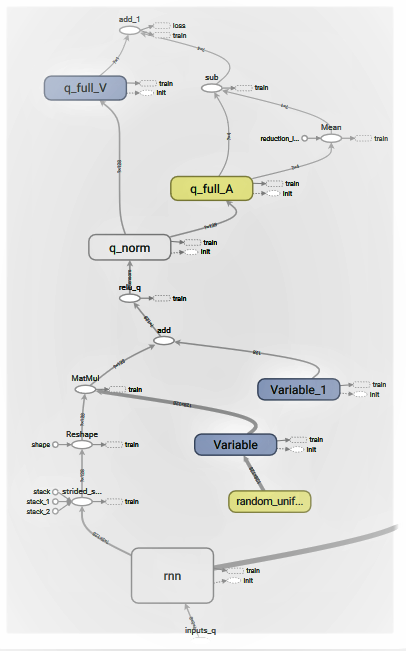
\includegraphics[width=0.25\textheight]{Q_net_tensorboard}}}
		\hspace{1em}
		\subfigure{\label{fig:tensorboard_q_target}}\addtocounter{subfigure}{-2}
		\subfigure{\subfigure[$Q_{target}$网络结构]{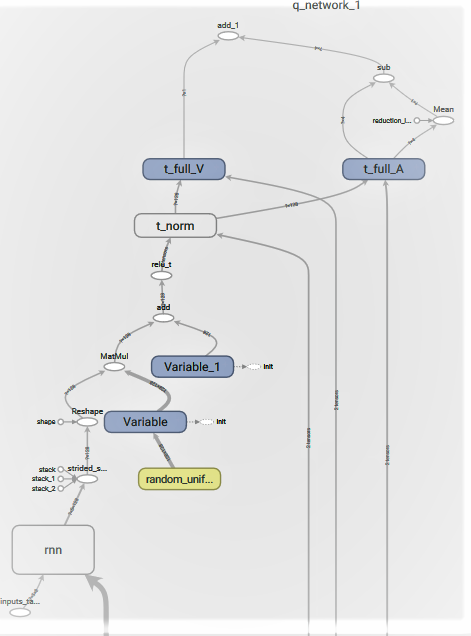
\includegraphics[width=0.3\textheight]{Q_target_net_tensorboard}}}
		\hspace{1em}	
	\end{minipage}
	\vspace{0.2em}
	\caption{Tensorboard中两网络结构图}\label{fig:target网络}
\end{figure}

\subsection{目标\textit{Q}网络}
加入dueling方法后的新型网络结构拥有了更短的训练时间和更高的更新速度,但整个系统的稳定性却达不到本文的预期要求。为此,通过借鉴DeepMind在2015年提出的一种新型算法对网络框架进行了更新和调整。这里本文在原有DRQN网络上再加上一个结构和初始权值一模一样的深度神经网络,两者分别使用$Q_{value}$和$Q_{target}$表示。在训练时本文会固定住$Q_{target}$网络的权值参数,仅对$Q_{value}$网络进行网络的反向梯度传递和权值更新,然后在经历固定次数(取决于本文设定的超参数)训练后将$Q_{value}$网络中所有权值和偏置参数复制给$Q_{target}$网络,达到一个延迟更新的目的。下面本文通过具体数学推导解释这样操作的原因。在计算网络的损失函数(TD error)时,本文是通过计算$Q_{value}$和$Q_{target}$的输出插值得到的,如式(\ref{eq:target weight})所示。
\begin{equation}\label{eq:target weight}
\Delta w=\alpha\left [ \left ( R+\gamma\max _{a} \hat{Q}\left ( {s}' ,a,w\right )\right )- \hat{Q}\left ( s ,a,w\right )\right ]\nabla_{w}\hat{Q}\left ( s,a,w \right )
\end{equation}


在实际计算中,本文希望公式(\ref{eq:Q学习更新函数})中$E_{k}$趋近于零,因此,令$Q_{value}$网络输出值为本文想逼近的\textit{Q}函数,$\gamma\max _{a} \hat{Q}\left ( {s}' ,a,w\right )$设为$Q_{value}$网络逼近的下一状态\textit{Q}函数,其加上奖赏$r(s,a)$形成训练标签。问题在于该标签中$\gamma\max_{a}\hat{Q}\left ( {s}' ,a,w \right )$部分同网络权值具有极大的相关性,也就是每次训练标签同训练目标向同一方向改变,会产震荡现象,影响训练收敛及其稳定性。因此本文需要额外引入一个固定的标签,也即$Q_{target}$网络形成的标签,使用独立的参数来预测TD-error,并在固定次数步骤后对权值进行复制来进行训练,如公式(\ref{eq:new target})所示。
\begin{equation}\label{eq:new target}
\Delta w=\alpha\left [ \left ( R+\gamma\max _{a} \hat{Q}\left ( {s}' ,a,w^{-}\right )\right )- 	\hat{Q}\left ( s ,a,w\right )\right ]\nabla_{w}\hat{Q}\left ( s,a,w \right )
\end{equation}

在代码层面实际操作时,本文需要构建两个相同结构网络,但分别放置于不同的命名空间下,以此做到权值的独立性,这里本文对其Tensorboard结构图\ref{fig:target网络}进行展示。

\section{本章小结}
在这一章中,本文对深度强化学中\textit{Q}学习,DQN以及LSTM进行了简要介绍,通过类比认知无线电同强化学习相似之处,给出使用机器学习解决频谱分配问题的方案,并依据LSTM的历史信息感知判断和DQN对于MDP问题的高效决策能力,引出解决频谱分配问题需要使用的DRQN结构,并在此基础上加入Dueling方法提高算法训练效率,使用固定的$Q_{target}$网络保证网络的稳定性。对论文所使用的算法进行概要介绍以及必要的数学推导,便于从原理上理解机器学习解决相关问题的底层原理,为后文结果展示给出所需的理论基础。

\chapter{异构通信系统频谱资源分配问题建模}
\section{引言}
异构系统这里指空天地一体化通信框架融合卫星通信,空基无人机(UAV),地面移动通信为一体,三者优劣互补,可为未来通信提供更广覆盖,更低延时,更大带宽,更高可靠的新一代通信服务。对于传统地面蜂窝网结构进行改进,提出基于分簇模型的新型框架,使用户在作为服务中心的同时成为资源分配中心,可以更自主,更便捷,也更高效合理的实现资源分配。本章将对空天地一体化模型进行展示,并着重介绍本文提出的分簇模型框架,并将对设计的相关问题的数学模型进行叙述。

\section{异构通信系统新型框架模型的建立}
对于现有传统通信系统如图\ref{fig:现有框架}所示。主要包括卫星通信系统,空基无人平台以及地面通信网络。其中地面段通信系统较为完善,而对于包含高空平流层的空天地一体化的通信系统模型研究还并不完善,这里本文需要对于异构系统进行简化。
\begin{figure}[h]
	\centering
	\includegraphics[width = 0.8\textwidth]{一体化框架}
	\caption{现实情况下异构系统通信框图}
	\label{fig:现有框架}
\end{figure}

简化后的模型如图\ref{fig:简化模型}所示。卫星可以直接与地面终端进行通信,同时也可以经由空中无人平台进行中转和广播,由于设计协议复杂,本文现就问题主要矛盾,即地面段异构系统的频谱分配进行研究,在算法较为成熟时再考虑空间段的具体细节。

\begin{figure}[h]
	\centering
	\includegraphics[width = 0.7\textwidth]{简化模型}
	\caption{简化后的新型通信框架}
	\label{fig:简化模型}
\end{figure}

\section{分簇模型}
\subsection{分簇模型结构}
这里不同于传统的蜂窝网概念,本文创新性的提出用户为中心自组织式的分簇模型。在本文构建的新型通信模型下,作为中介节点的不止有基站,可能还有一些设备能力较强的终端用户形成自组织式的小小区,本文将之称为簇头,现在主要讨论簇内与簇间在考虑同频干扰情况下的频谱分配算法的优化。

模型构建类似于地面移动通信的蜂窝网模型,但与之不同点在于基站的角色由簇头承担,簇头可以是具有较强计算能力的移动终端,也可以是现存基站,分簇模型如图\ref{fig:分簇模型结构图}所示。

这里本文假设每个簇头可能连接多个簇内用户为他们提供信息传输服务,每个用户也可能同时连接多个簇头,通过训练后的分布式智能体( 簇内用户)可以自主选择连接哪些簇头,然后在被告知共用用户数量后再自主选择特定信道申请分配。

这些都结束后,中心智能体(簇头)会根据申请连接情况进行智能功率控制,以此达到网络总传输速率最高。
\begin{figure}[h]
	\centering
	\includegraphics[width = 0.9\textwidth]{分簇模型结构图}
	\caption{分簇模型结构示意图}
	\label{fig:分簇模型结构图}
\end{figure}

\subsection{分簇模型建立原因及意义}
关于分簇原因本文这里列出如下:

(1) 动态的网络:用户和基站都将具有相当的移动性。用户的移动性不再赘述,基站的移动性主要是指一体化组网构架下,为了弥补地面网络带宽受限的问题而引入了平流层的飞艇作为移动的基站。在这种状况下,不得不通过分簇来解决动态性的问题。

(2) 分布式的系统:未来系统可能是分布式的,之前的工作也已经说明,分布式系统中的用户联系松散,需要根据特定的情况来保持和特定用户群体的联系。因此,分簇和分布式的系统也是密切相关的。

(3) 用户需求多样化的网络:用户对通信的需求大相径庭,需要打破小区不重叠、 在哪个小区用哪个基站的限制,让用户自由选择节点、甚至组成以自己为中心的簇,自主地调配资源,为自己服务。

\section{问题的数学模型}
这里本文对相关问题进行简化和抽象,并进行数学建模,为后续问题解决提供体系化的理论支持。首先本文给出整个问题的完整流程图如\ref{fig:整体流程图}所示。待解决问题主要分为三个部分,实现簇头自主选择部分,本文简化问题为基于历史信息的相关信道状态预测问题,定义为部分观测的马尔可夫决策过程(POMDP)。然后是实现分布式多用户冲突避免问题,本文建模为纳什均衡问题,也称非合作博弈均衡,在仅知道竞争用户数量情况下通过训练使智能体达到纳什均衡状态。
\begin{figure}[htbp]
	\centering
	\includegraphics[width = 0.9\textwidth]{分簇频谱分配算法}
	\caption{异构系统频谱智能分配整体流程图}
	\label{fig:整体流程图}
\end{figure}

最后是功率控制部分,本文建模为认知无线电下次级用户的功率退避问题。

对于簇头的选择是用户依据历史信息对不同簇头当前转发状态与能力的估计,在之前的时隙中(timeslot),用户在每个时间隙发出信息传输请求,得到信息传输结果观测值(ACK),以此估计当前簇头转发状态好坏,输出一个布尔值(0/1),这里假设不同簇头之间是相关的,由于不能完全知晓当前簇头状态转移模式,因此是一个部分观测马尔可夫决策过程,如表格\ref{tab:马尔可夫分类}所示。对于挑选簇头问题可以建模为一个$2^{N}$状态的马尔科夫链,\textit{N}表示用户可连接簇头数目,状态空间为$S=\left\{S_{1},\cdots,S_{2^{N}}\right\}$,其中每个$S_{i}$,为一个长度为\textit{N}的向量,表示每个簇头当前状态。用户通过历史信息进行预测,并更新自身的系统状态分布推测$\Omega \left ( t \right )=\left [ \omega _{S_{1}} \left ( t \right ),\cdots,\omega _{S_{2^{N}}} \left ( t \right )\right ]$,每个向量元素表示系统位于当前状态概率,并依据此估计给出最优动作选择向量$a(t)$并获取ACK,以此根据公式(\ref{eq:簇头选择更新公式})(式中$\mathbb{I}\left(\cdot\right)$为指示函数)更新系统状态猜测向量\cite{8303773}。
\begin{equation}\label{eq:簇头选择更新公式}
\hat{\omega }_{S_{i}}\left ( t \right )=\left\{
\begin{aligned}
\frac{\omega _{s_{i}\left ( t \right )}\mathbb{I}\left ( S_{ik}\left ( t \right ) =1\right )}{\sum_{i=1}^{2^{N}}\omega _{s_{i}\left ( t \right )}\mathbb{I}\left ( S_{ik}\left ( t \right ) =1\right )}& & a(t)=k,o(t)=1\\
\frac{\omega _{s_{i}\left ( t \right )}\mathbb{I}\left ( S_{ik}\left ( t \right ) =1\right )}{\sum_{i=0}^{2^{N}}\omega _{s_{i}\left ( t \right )}\mathbb{I}\left ( S_{ik}\left ( t \right ) =0\right )}& & a(t)=k,o(t)=0
\end{aligned}
\right.
\end{equation}

然后将猜测向量与每个簇头不同概率分布组成的状态转移矩阵\textit{P}做乘积得到下一状态概率矩阵$\Omega \left ( t+1 \right )$,以此达到长期累积折扣奖赏最大的优化目标,获得最优策略,如公式(\ref{eq:簇头选择长期奖励})所示。其中$R_{\pi\left ( \Omega \left ( t \right ) \right )}\left ( t \right )$为t时刻在当前状态$\Omega \left ( t \right ) $下,最佳策略$\pi^{*}$采取动作后得到的奖赏。折扣因子$\gamma$为介于0和1之间的数,用来表示长期奖励对总任务的重要程度。
\begin{equation}\label{eq:簇头选择长期奖励}
\pi ^{*}= \underset{\pi }{\arg \max}\mathbb{E}_{\pi}\left [ \sum_{t=1}^{\infty }\gamma ^{t-1} R_{\pi\left ( \Omega \left ( t \right ) \right )}\left ( t \right )\mid \Omega \left ( 1 \right )\right ]
\end{equation}

当簇头间相互独立且簇头状态转移概率分布形式一致时,每个用户基于自身的贪心算法即为最优策略\cite{Ahmad2009Optimality},但对于簇头间相互关联且变化概率分布未知的情况下这种算法得到的结果并不是最优化的,且由于簇头间相关性,该问题为一个PSPACE-hard问题\cite{8303773},很难通过传统算法得到精确解。
\begin{table}[htbp]
	\caption{马尔可夫模型类别}\label{tab:马尔可夫分类}
	\vspace{0.5em}\centering\wuhao
	\begin{tabular}{cccc}
		\toprule[1.5pt]
		名称 & 状态可见性 & 是否考虑动作 & 英文缩写 \\
		\midrule[1pt]
		马尔科夫链 & 状态完全可见 & 不考虑动作影响 & MC \\
		马尔可夫决策过程 & 状态完全可见 & 考虑动作影响 & MDP\\
		隐马尔可夫模型 & 状态不完全可见 & 不考虑动作影响 & HMM \\
		部分观测马尔可夫决策过程 & 状态不完全可见 & 考虑动作影响 & POMDP \\
		\bottomrule[1.5pt]
	\end{tabular}
\end{table}


对于分布式多用户对有限信道的竞争问题建模为纳什均衡问题。这里给出纳什均衡的定义在博弈$ G=\left \{ S_{1},\cdots,S_{n}:U_{1},\cdots,U_{n}\right \}  $中,每个博弈方采取一个策略,组成一个策略集合$\left\{S_{1}^{*},\cdots,S_{n}^{*}\right\}$,对于其中任意一个博弈成员$i$的策略$S_{i}^{*}$都是对其余博弈者采取策略组合$\left\{S_{1}^{*},\cdots,S_{i-1}^{*},S_{i+1}^{*},\cdots,S_{n}^{*}\right\}$的最佳应对策略,也即$U_{i}\left \{ S_{1}^{*}, \cdots ,S_{i}^{*},\cdots,S_{n}^{*} \right \}\geqslant U_{i}\left \{ S_{1}^{*},\cdots ,S_{ij}^{*},\cdots,S_{n}^{*} \right \}$对于任意$S_{ij}\in S_{i}$恒成立,本文称对应的策略集合为$G$的一个纳什均衡。通俗来讲就是其他竞争对手不改变自身竞争策略时候,自己不改变当前策略才会获取利益最大值,也就是达到平衡状态。对于信道竞争问题来说,即为在分布式用户间不进行合作式信息交流前提下达到平衡状态的问题。这里本文使用$\mathcal{N}=\left \{ 1,2,\cdots,N \right \}$表示簇内竞争用户然后使用集合$\mathcal{K}=\left \{0,1,2,\cdots,K \right \}$表示选择的信道(如果选择动作为0则表示用户在此时隙选择避让,不进行信息传递),在每个时隙,同一簇内不同用户选择一个簇头可提供信道发出信息传输请求,如果和其他用户不发生冲突则返回成功传输信号(ACK),反之亦然。目标仍然是达到长期总传输成功率最高。这里本文仍然使用带有折扣系数$\gamma$的累积奖赏作为优化目标,如式(\ref{eq:冲突避免奖赏公式})所示。
\begin{equation}\label{eq:冲突避免奖赏公式}
R_{n}=\sum_{i=1}^{N}\sum_{t=1}^{\infty }\gamma ^{t-1}r_{n}\left ( t \right )
\end{equation}

由于用户间不能相互通信,所以普通算法对于这种问题只能使用随机信道选取方式,导致信道出现空闲或冲突,致使频谱利用效率降低,本文将使用深度强化学习解决这一问题。

对于多用户功率功率控制问题,本文将其设定为在认知无线电框架下的次级用户的功率退避问题。在完成簇头选择和信道选择后,簇头和簇内用户成功建立通信链路,但由于多用户的存在以及用户移动变化等因素,如果不采取相应的动态功率控制肯能导致同频干扰或是邻频干扰对信息传递造成巨大干扰,降低通信服务质量。简化起见,本文考虑簇内有2个用户,并将其中一个假设为主用户(PU),另一个为次级用户(SU),且每个用户都拥有自己的发射机($T_{X_{1}},T_{X_{2}}$)与接收机($R_{X_{1}},R_{X_{2}}$),主用户不需要考虑次级用户,并且仅依据自己固定的原有功率策略进行功率调整。次级用户需要通过感知周围环境对主用户功率变化产生响应,及时调整自己的功率参数,以达到共同通信目的。虽然主用户与次级用户不产生直接信息交流,但次级用户功率调整会通过环境变化引起主用户做出功率改变,也即客观上两者会产生相互作用。方便起见,本文假设两者同步进行功率调整,拥有相同时间基线。同时有感应节点部署在环境中获取接收信号强度(RSS, received signal stength),协助次级用户估计主用户传输状态。本文使用信干噪比SINR表示各用户QoS,如公式(\ref{eq:SINR})所示,式中$h_{ij}$表示对应信道增益,$N_{i}$为对应噪声功率,主用户功率策略\cite{Grandhi1998Constrained}为如下公式所示(\ref{eq:传统功率策略})。式中$D\left ( \cdot  \right )$为离散式功率选择函数,选取离散功率集合以$\mathcal{P}_{1}\triangleq\left \{ p_{1}^{p},\cdots,p_{L_{1}}^{p} \right \}$表示。$SINR_{1}(k)$为主用户测量得到的信干噪比,$p_{1}(k)$为主用户选择的功率。环境状态使用$p_{n}^{r}(k)=p_{1}(k)g_{1n}+p_{2}(K)g_{2n}+w_{n}(k)$进行描述,$p_{1}(k)g_{1n},\;p_{2}(K)g_{2n}$分别表示两用户发射功率同各自增益乘积,$w_{n}(k)$表示零均值高斯白噪声。
\begin{equation}\label{eq:SINR}
SINR_{i}=\frac{\left \| h_{ii} \right \|^{2}p_{i}}{\sum_{j\neq i}\left \| h_{ji} \right \|^2p_{j}+N_{i}}\; i=1,2 
\end{equation}
\begin{equation}\label{eq:传统功率策略}
p_{1}\left ( k+1 \right )=D\left ( \frac{\eta _{1}p_{1}\left ( k \right )}{SINR_{1}\left ( k \right )} \right )
\end{equation}

随后次级用户在智能体决策下选择一个功率集合$\mathcal{P}_{2}\triangleq\left \{ p_{1}^{s},\cdots,p_{L_{2}}^{s} \right \}$中的功率进行信息传输。当两用户都满足QoS要求($SINR_{i}\geqslant\eta_{i}$)时,此时刻返回奖赏为1,最终目标为整体长时累积奖惩最大化。
\section{本章小结}
在这一章节中,本文对整个问题的背景框架以及整体算法流程进行了介绍,并提出一种基于分簇理论的新型通信框架,在此基础上对于问题涉及的簇头选择,信道分配,功率控制这三方面进行了具体的数学语言描述,分别建模为部分观测马尔可夫决策过程,纳什均衡问题以及认知无线电框架下次级用户的功率退避问题,形成一个完备严密的数学体系,为后续工作提供理论指导。









\chapter{异构通信系统频谱智能分配}
\section{引言}
在介绍了使用的机器学习算法及问题背景和数学模型之后,本章将对于基于分簇模型的异构系统频谱智能分配问题分为簇头选择,信道选择,功率控制三方面进行具体阐述以及使用Python配合Tensorflow平台进行算法仿真验证的结果展示以及分析,最后对本文使用的算法进行性能评估,提出存在不足并指出后续工作方向。

\section{DRQN算法流程及代码实现}
在结合LSTM网络结构以及DQN算法基础上形成的DRQN网络,并对其进行Dueling和加入$Q_{target}$网络操作后本文给出一个完整DRQN的算法,如算法\ref{alg:DRQN}所示。
\begin{algorithm}[htb]  
	\caption{带有目标网络及经验回放策略的DRQN算法 }  
	\label{alg:DRQN}  
	 \begin{algorithmic}[1]  
		\Require  
		可交互环境类$ENV$;DRQN智能体$Agent$;储存体$Memory$;  
		\Ensure  
		智能体选取的输出动作集合$action$;  
		\State 初始化储存体$Memory$; 初始化智能体$Agent$中$Q_{value}$和$Q_{target}$网络的权值参数$w$和$w^{-}$;
		初始化环境状态,以随机动作方式生成输入状态$s_{t}$; 
		\State 将状态输入DRQN网络中,获取动作价值向量$Q$;  
		\State 使用前文介绍的$\epsilon -$贪心算法选取动作$a_{t}$; 
		\State 将该动作输入环境交互器$ENV$,获取动作对应奖励$r$,并生成下一状态$s_{t+1}$;
		\State 令$s_{t}=s_{t+1}$;将$s_{t},a_{t},r_{t},s_{t+1}$存入储存体中; 
		\State 当储存体中数据长度达到训练要求时开始网络训练过程; 从储存体中随机抽取固定数量的历史数据;  
		\State 将$s_{t}$输入$Q_{value}$网络,得到$Q$值;将$s_{t+1}$输入$Q_{target}$网络,加上$r_{t}$得到$target$值;
		\State 利用公式(\ref{eq:new target}),$\Delta w=\alpha\left [ \left ( R+\gamma\max _{a} \hat{Q}\left ( {s}' ,a,w^{-}\right )\right )- 	\hat{Q}\left ( s ,a,w\right )\right ]\nabla_{w}\hat{Q}\left ( s,a,w \right )$计算权值的反向传播梯度;
		\State 使用ADMA优化器进行$Q_{value}$网络的$w$更新;
		\State 每隔固定训练次数$n$就将$Q_{value}$网络的$w$传递给$Q_{target}$网络的权值参数$w^{-}$;
		\State 重复上述2至10操作至任务结束; \\
		\Return $Action$,$r$的累积奖赏$reward$;  
	\end{algorithmic}  
\end{algorithm}  

在使用Python3.6具体实现相应代码时,我将智能体设置成‘类’形式(Class),将函数和参数初始化包含在类中,借助Tensorflow编写神经网络搭建部分,利用张量间的矩阵乘法与加法实现全连接神经网络的构建。对于记忆体部分采用字典形式进行智能体与环境交互过程信息的储存,采取堆栈弹出和随机读取方式实现之前提到的经验回放策略。至于反向训练部分,使用Tensorflow自带的Adma优化方式进行梯度的反向传播,并进行神经元参数的训练,在网络收敛后结束训练循环。随后将结果使用Pandas工具转换为.csv为后缀的数据文件储存,通过matplot.pyplt函数库绘制性能曲线,并进行分析。

\section{簇头选择}
\subsection{基于DRQN的簇头选择}
根据前文叙述的内容,用户在分簇模型下首先要在备选连接簇头集合$\mathcal{H} \triangleq \left \{ h_{1} ,h_{2},\cdots,h_{n}\right \}$中,依据自身信号传输要求选取最适合自身的相应簇头$h_{i}^{*}$,与之建立通信链路,进行信息传递。算法性能选用一定时间后用户自身传输信息成功比例表示,同时本文使用随机选择方式在备选簇头中任意选取簇头进行通信链路建立,统计同等情况下算法成功率。这里比较特殊的一点是不同簇头的状态变化间是相关的,这个设定主要考虑分簇模型中一些移动用户也会成为潜在簇头,由此不同于传统地面基站作为中介节点的蜂窝网构架下不同基站间相互影响由于距离较大的因素较小,所以可以忽略基站间影响。

\begin{algorithm}[htb]  
	\caption{簇头相关动态状态转移算法}  
	\label{alg:headstate}  
	\begin{algorithmic}[1]  
		\Require  
		可用簇头集合$\mathcal{H}$;状态转移概率$P$; 划分集合数$K$; 
		\Ensure  
		备选簇头状态向量$S$;  
		\State 初始化随机簇头分配集合$\mathcal{T}\triangleq\left \{ t_{1}\triangleq\left \{h_{a},\cdots,h_{b}\right \} ,\cdots,t_{K}\triangleq\left \{h_{c},\cdots,h_{d}\right \}\right \}$;
		\State 随机选取一个集合为初始簇头激活集合,如$t_{i}$;				
		\State 在每个时隙开始时,生成一个随机数$\epsilon$,如果$\epsilon>P$,将当前激活集合取消激活,激活下一集合$t_{j}$;反之保持当前状态;  
		\State 将该时隙全部簇头状态存入簇头状态向量中;
		\State 重复上述3,4操作,至任务结束; \\
		\Return 簇头状态向量$S$;  
	\end{algorithmic}  
\end{algorithm}  

但对于本文的分簇模型,不同小簇头间距离较近,且可能进行业务协同,由此必须假定不同簇头间是紧密相关的,对于这种相关的多簇头未知变化规律的预测问题需要让智能体通过历史信息获得预测当前状态的能力,同时有需要让智能体拥有长期奖赏最大化的决策能力,无疑前文介绍的DRQN方法是最合适的解决工具。

具体实现多簇头联合相关状态变化这一目的,本文借鉴已有文章的思路\cite{8303773},进行簇头状态相关性变化构造。进行仿真时,本文假设有16个备选簇头,将这些簇头随机划分到几个子集中,并将转移概率固定为$P=0.9$,最初状态下随机假定一个集合为活跃簇头集合,该集合内所有簇头均为可用的,活跃的,用户选取相应簇头进行信息传输时可以得到成功反馈($ACK=1$),在每个时隙开始前,活跃集合序号会依据固定的转移概率按照事先规定好的随机顺序转移至下一序号对应的簇头集合,激活其中所有簇头,以此实现簇头的相关动态状态转变,如算法\ref{alg:headstate}所示。


按照这种算法本文生成簇头状态图,如图\ref{fig:簇头状态}所示。

图中选取前15个时隙作示意。图中可以明显看到簇头间变化的相关性,比如簇头10和簇头11变化规律一致,6和7变化规律一致。且可以看出簇头变化是较为剧烈的,这对于不知道簇头变化规律的申请用户来说想实现连续成功接入是较为困难的,但通过使用DRQN网络则可以较为出色的完成这一任务。
\begin{figure}[htbp]
	\centering
	\includegraphics[width = 0.9\textwidth]{簇头状态}
	\caption{相关簇头状态变化示意图}
	\label{fig:簇头状态}
\end{figure}


\subsection{簇头选择结果展示及分析}
在完成簇头变化状态建立之后需要对DRQN网络输入和输出进行调整,并使其可以同本文编写的环境模型进行交互。本文设置仿真超参数如表\ref{tab:超参数}所示。
\begin{table}[htbp]
	\caption{DRQN网络超参数设置}\label{tab:超参数}
	\vspace{0.5em}\centering\wuhao
	\begin{tabular}{cc}
		\toprule[1.5pt]
		超参数名称 & 仿真设置值 \\
		\midrule[1pt]
		探索概率$\epsilon$ & 0.1 \\
		训练单批次数据量 & 64\\
		LSTM时间步长 & 5 \\
		全连接层数 & 3 \\
		全连接层节点数 & 200 \\
		全连接层激活函数 & ReLU \\
		学习率 & $10^{-5}$ \\
		折扣因子$\gamma$ & 0.85 \\
		\bottomrule[1.5pt]
	\end{tabular}
\end{table}

本文将此前$K$步采取的动作和得到的传输反馈合并为一个向量做为状态输入DRQN中,动作输出设置为当前状态下预测信道序号,奖赏对应于采取该信道进行通信时成功与否的(ACK)反馈信息。然后使用算法\ref{alg:DRQN}开始仿真。同时给出随机选择方式结果用以对比算法性能。首先利用Tensorboard工具给出训练过程中的损失函数图\ref{fig:簇头训练loss}。 
\begin{figure}[htbp]
	\centering
	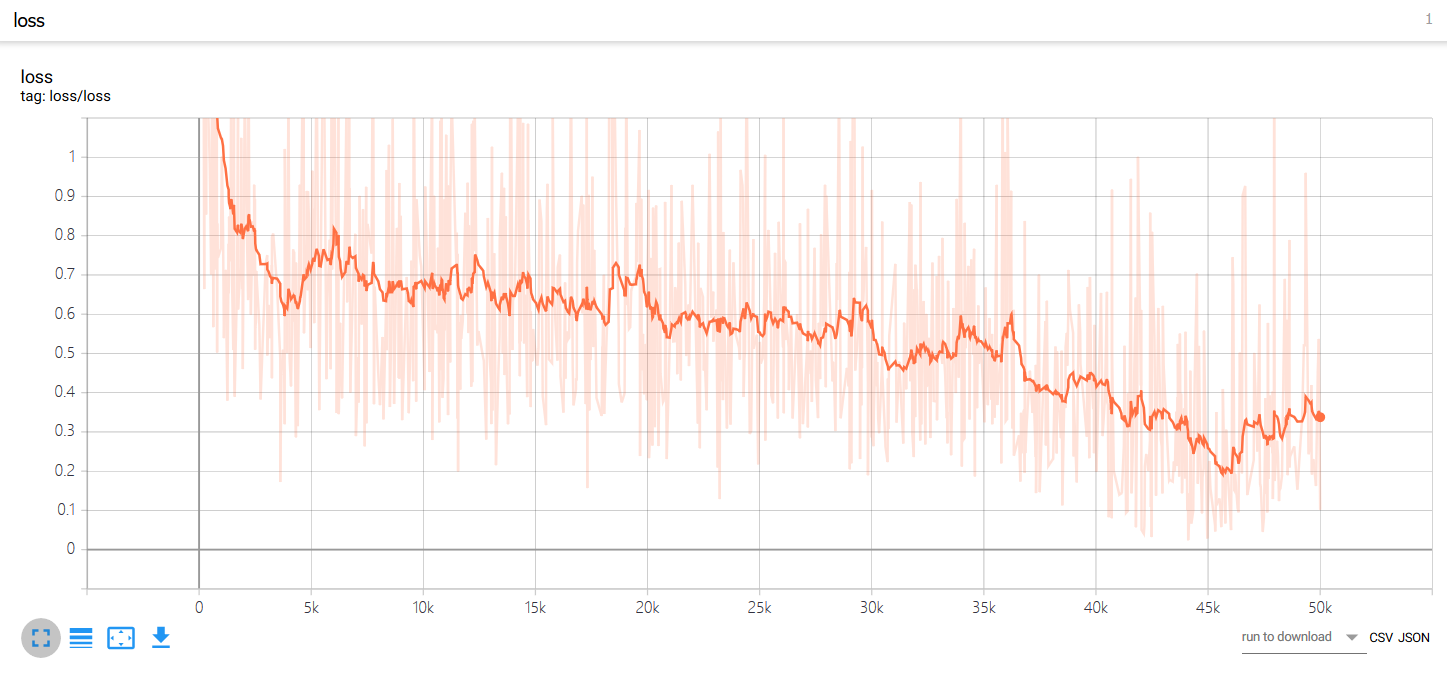
\includegraphics[width = 1\textwidth]{频道选择,损失,tensorboard}
	\caption{Tensorboard训练损失曲线图}
	\label{fig:簇头训练loss}
\end{figure}

由训练损失曲线可以看出随着训练次数的增加,训练损失逐渐降低,表明本文的训练是较为有效的,此外,在训练结束后对网络模型进行验证时损失曲线稍有上升,我的理解是训练有轻微过拟合问题导致的负增益,但这仍是可接受的,下面对输出结果进行展示,并对算法性能进行分析。

首先本文给出两种算法给出的簇头选择,对于DRQN智能体给出的结果具有十分明显的簇头倾向性,表明智能体通过对于历史信息的学习对于簇头状态拥有自己的判断,相比于随机算法的选择显然是更为合理的。如图\ref{fig:簇头动作对比}所示。

\begin{figure}[htbp]
	\begin{minipage}{\textwidth}
		\centering
		\subfigure{\label{fig:簇头动作DRQN}}\addtocounter{subfigure}{-2}
		\subfigure{\subfigure[DRQN算法的簇头选择展示]{\includegraphics[width=0.5\textheight]{簇头动作DRQN}}}
		\hspace{1em}
		\subfigure{\label{fig:簇头动作random}}\addtocounter{subfigure}{-2}
		\subfigure{\subfigure[random算法的簇头选择展示]{\includegraphics[width=0.5\textheight]{簇头动作random}}}
		\hspace{1em}	
	\end{minipage}
	\vspace{0.2em}
	\caption{随机算法同DRQN算法选取簇头对比}\label{fig:簇头动作对比}
\end{figure}

\begin{figure}[htbp]
	\centering
	\includegraphics[width = 0.7\textwidth]{簇头条形图}
	\caption{DRQN及随机算法簇头选择概率情况}
	\label{fig:簇头条形图}
\end{figure}

这里本文给出不同簇头在两种算法下的选取统计概率,对于个别簇头高概率选取的策略是否有效需要通过两种算法不同的信息传输成功情况来体现。因此本文给出两种算法对于同一情况给出的不同选择的传输反馈(ACK)来表示,图\ref{fig:簇头对比折线}展示随时间进行,使用DRQN算法的智能体累积奖赏值高于随机选取算法。具体传输结果如图\ref{fig:簇头奖励对比}所示。图中绿色方格代表用户在该时刻成功选择了合适的簇头,成功进行簇头用户间链接,可从肉眼直观看出使用DRQN算法的簇头选择策略成功率显著高于使用随机选取方式的智能体。这也证明了本文的算法是有效果的,进行了正向优化。
\begin{figure}[htbp]
	\centering
	\includegraphics[width = 0.7\textwidth]{簇头对比折线}
	\caption{DRQN同随机算法簇头选择成功率对比曲线}
	\label{fig:簇头对比折线}
\end{figure}

\begin{figure}[htbp]
	\begin{minipage}{\textwidth}
		\centering
		\subfigure{\label{fig:簇头奖励DRQN}}\addtocounter{subfigure}{-2}
		\subfigure{\subfigure[DRQN算法的簇头选择展示]{\includegraphics[width=0.5\textheight]{簇头奖励DRQN}}}
		\hspace{1em}
		\subfigure{\label{fig:簇头奖励random}}\addtocounter{subfigure}{-2}
		\subfigure{\subfigure[random算法的簇头选择展示]{\includegraphics[width=0.5\textheight]{簇头奖励random}}}
		\hspace{1em}	
	\end{minipage}
	\vspace{0.2em}
	\caption{随机算法同DRQN算法选取簇头成功情况对比}\label{fig:簇头奖励对比}
\end{figure}


\section{信道选择}
\subsection{基于DRQN的分布式用户信道选择}
在每个用户都选取自己理想连接簇头后,就需要执行信道分配动作。因为一个小簇头可提供信道数量并不太多,在用户饱和场景下难免会产生信道申请冲突,用户竞争信道会导致双方信息传输失败,致使信道利用效率大大降低,因此用户间的冲突避免就显得尤为重要。由于是异构通信框架下的资源分配,不同用户可能分属于不同的网络系统,因此这里本文需要假设用户间不进行信息交流,在这种情况下如果使用中央分配方式可以轻松解决该问题,但本文构建的分簇模型中簇头除了地面固定基站外还可以是空中无人机平台(UAV)以及地面段部分用户,这时如果将信道分配工作全部交由中心节点进行处理和组织,会给簇头带来较大的计算任务负担,影响其信息传输业务。其次,由于本文考虑的是多用户动态频谱分配,用户具有移动性,进行中央式频道管控面临频繁的分配策略变更问题,任意用户进出都将要求中心节点进行重新规划和分配,在簇头和用户高密度的未来通信场景下显然是不利的。这里本文需要采取分布式智能方式,自主选择申请信道,并配合自身的簇头选择完成完全以用户自身为中心的自主化资源申请与分配。这样可以充分体现分布式策略优势,同时也最大化分簇模型的用户QoS体验,实现每个用户都成为"中心"的资源分配思想。
\begin{figure}[htbp]
	\centering
	\includegraphics[width = 0.7\textwidth]{信道动作随机}
	\caption{随机算法下用户选择信道结果}
	\label{fig:信道随机动作}
\end{figure}

分布式智能决策设定让用户在对其他用户选择频道未知状态下如何做出最优信道选择被建模为一个经典的纳什均衡问题。在这种信息不对称情况下进行动作选择颇为困难,首先本文给出随机选取方式下的信道分配结果。进行仿真时为简便起见本文设置三个竞争用户,共同分配两个可用信道($channel_{1},channel_{2}$),每个用户在每个时隙选择一个自己的申请信道动作,这里本文用($0,1,2$)来表示,其中$0$表示用户在当前时隙状态下不进行信息传递,选择避让,$1$和$2$则表示选取对应信道进行信息传输,结果如图\ref{fig:信道随机动作}所示。对冲突信道申请检测并判定为信息传输失败,对不冲突的信道选择进行统计,结果如图\ref{fig:信道成功随机}所示。
\begin{figure}[htbp]
	\centering
	\includegraphics[width = 0.7\textwidth]{信道成功随机}
	\caption{随机算法下用户选择信道成功结果}
	\label{fig:信道成功随机}
\end{figure}

显然,用户任意选择会导致大量冲突产生,降低频谱效率,这时本文就需要DRQN算法进行智能体训练及优化。在应用DRQN算法解决该问题时,本文仍然将多步历史决策动作和观测信息结果作为网络的输入,将选取的申请信道作为动作,将该动作是否与其他用户发生冲突作为反馈信息,也即奖励。进行具体仿真时使用DRQN算法,如算法\ref{alg:DRQN}所示。但是这里在具体仿真时出现了一些问题,比如使用整体网络累计奖赏作为每个用户评价指标时,本文成为用户合作模式,在该模式下会出现某一用户始终选择回避,不进行信息传递,这显然是不公平的,为此本文对单个用户训练时奖赏值进行修改,使其训练时使用竞争模式,这样在最终整体网络总传输效率不变的情况下,可以最大程度满足用户间的公平性。

且在使用$DRQN$算法进行训练时,训练数据馈入方式也需要进行改变,自然的馈入数据的组织形式为如式(\ref{eq:size1})所示。
\begin{equation}\label{eq:size1}
DATA=\left[\left(Batch\_size \right),\left(User\_num \right),\left(Time\_step \right),\left(State\_size \right)\right]
\end{equation}

这样训练出来的算法偏向于合作模式,这时本文需要对数据进行重新的整理和分组,将单个用户特征进行凸显,将数据格式重组为如式(\ref{eq:size2})所示。
\begin{equation}\label{eq:size2}
DATA=\left[\left(User\_num \right),\left(Batch\_size \right),\left(Time\_step \right),\left(State\_size \right)\right]
\end{equation} 

使同一用户训练趋势固定,更容易达到竞争模式的平衡状态。具体仿真时仍使用表格\ref{tab:超参数}给出的仿真超参数,训练损失曲线通过Tensorboard展示,如图\ref{fig:loss_tensorboard}所示。

\begin{algorithm}[htb]  
	\caption{用户竞争奖赏算法}  
	\label{alg:headstate}  
	\begin{algorithmic}[1]  
		\Require  
		可用信道集合$\mathcal{H}$; 
		\Ensure  
		信道选取动作向量$S$;  
		\State 依据DRQN算法选取某一信道作为申请信道$h_{i}^{*}$;
		\State 使用该信道进行信道申请;				
		\State 在于环境交互后获取ACK反馈;  
		\State 对于成功传输信号的选择奖赏值设置不变,对于规避动作产生的其他用户成功信息传递自身奖赏$r=r-1$;
		\State 重复上述1至4操作,至任务结束; \\
		\Return 信道选取动作向量$S$; 总累计奖赏$reward$; 
	\end{algorithmic}  
\end{algorithm}  


\begin{figure}[htbp]
	\centering
	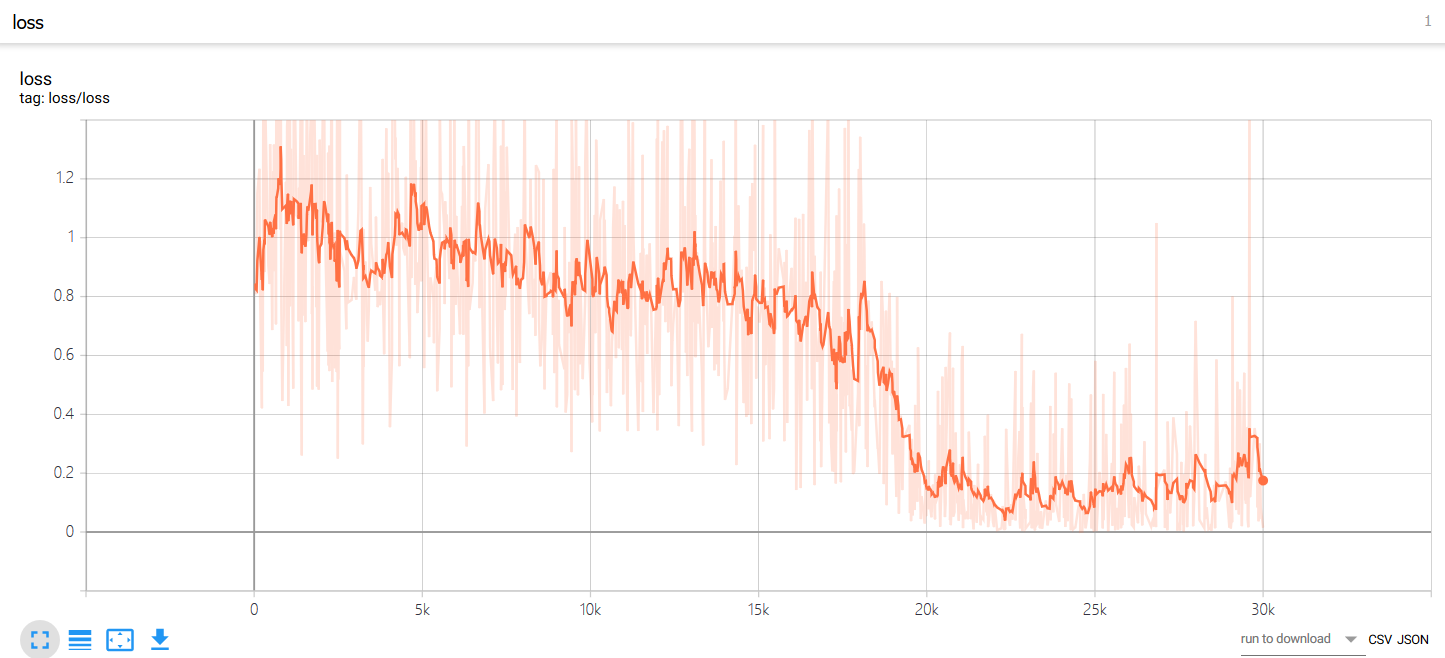
\includegraphics[width = 1\textwidth]{loss_tensorboard}
	\caption{DRQN算法Tensorboard损失曲线图}
	\label{fig:loss_tensorboard}
\end{figure}
\subsection{信道选择结果展示及分析}
首先给出使用合作式训练方法的得到的信道分配结果,如图\ref{fig:信道动作合作}所示。
\begin{figure}[htbp]
	\centering
	\includegraphics[width = 0.8\textwidth]{信道动作合作}
	\caption{DRQN合作型算法下用户选择信道结果}
	\label{fig:信道动作合作}
\end{figure}

从结果图中可以很直观的看出有两个用户长时间占用两个固定信道,有一个用户在大部分时间选择退避,不进行信息传递,显然,这样做可以使这两个信道不出现竞争冲突,频谱利用率极高。

然而,根据本文日常生活经验可知,这种信道分配策略显然是不合理的,对于三个用户分配有失公允,虽然达到初始设置目标但本文认为这种方法不可取。
\begin{figure}[htbp]
	\centering
	\includegraphics[width = 0.8\textwidth]{信道动作竞争}
	\caption{DRQN竞争型算法下用户选择信道结果}
	\label{fig:信道动作竞争}
\end{figure}

为此本文使用上文提到的竞争型DRQN算法,每个用户都将自身累积传输奖赏最大值设为训练目标,重新进行训练,得到如图\ref{fig:信道动作竞争}所示结果。从图中可以看出在最终目标不变的情况下本文得到了一个比较有趣的结果。

从图中可见用户1大概率占用信道1,剩余两用户竞争剩余的信道2,两者以类似于时分多址(TDMA)形式共用信道2,两者轮流进行自主退避,由此达到总传输奖赏最高,形成一种不完全的纳什均衡状态。结果可解释性较高,虽然三用户未实现完全绝对公平的信道分配,但对比合作型DRQN已经有较大程度的提升。

最后本文给出随机算法同本文使用的DRQN竞争型算法性能对比,如图\ref{fig:信道奖励对比}所示。可见DRQN算法优势明显。
\begin{figure}[htbp]
	\centering
	\includegraphics[width = 0.7\textwidth]{信道奖励对比}
	\caption{DRQN竞争型算法同随机算法性能对比结果}
	\label{fig:信道奖励对比}
\end{figure}

\section{功率控制}
\subsection{基于DRQN的智能化功率控制}
在用户结束了簇头选择以及信道选择成功建立同簇头间的通信链路之后,频谱分配任务还未结束,因为频点分配同时还应对于用户于簇头间通信功率进行控制,功率调节与信道选择休戚相关,不能分离。在进行功率控制任务时,本文仍然使用DRQN算法以及相同的网络构架。简便起见,本文只考虑两个用户在分簇模型中认知无线电框架下的次级用户功率退避问题。本文借用认知无线电中主用户和次级用户的概念进行功率问题研究,假设主用户使用固定功率调整策略如公式(\ref{eq:传统功率策略})所示,出于通信安全性考虑,需要保护每个用户的通信隐私,次级用户不能直接向主用户询问通讯功率,需要通过传感器信息预测分析主用户功率,并在不影响主用户前提下选择合适的通讯功率进行通信,以减小同频干扰(当用户数量过饱和时,可能会允许多用户使用同一频道情况)或邻频干扰(用户使用邻近频道情况)。在进行仿真测验时,本文将传感器信息设置为网络输入状态,两用户物理距离采取随机产生方式生成,且只考虑自用空间损耗和高斯白噪声影响。将次级用户选取的离散功率序号作为输出动作,并对两用户使用的通信功率同初始设定SINR阈值进行对比,返回两用户传输成功数据作为奖赏反馈。仿真时超参数设置同前表\ref{tab:超参数}所示。首先本文给出DRQN网络训练的损失曲线随训练次数的变化关系,如图\ref{fig:功率loss}所示。

\begin{figure}[htbp]
	\centering
	\includegraphics[width = 0.7\textwidth]{Loss}
	\caption{DRQN算法训练损失曲线}
	\label{fig:功率loss}
\end{figure}

\begin{figure}[htbp]
	\centering
	\includegraphics[width = 0.7\textwidth]{Success}
	\caption{DRQN算法测试成功率曲线}
	\label{fig:功率success}
\end{figure}
\subsection{功率控制结果展示及分析}
为了展示训练后智能体功率控制效果,本文引入两个比较参数,首先是$Success=\frac{success\_number}{test\_number}$用来表示使用算法可以最终达到理想共存状态$SINR_{i}\geqslant\eta_{i}$的成功比例,结果如图\ref{fig:功率success}所示。

可见随训练进行成功率整体上升,但稍有些不稳定。第二个参数$Used\_step$表示每次尝试从初始状态达到理想共存状态时需要使用的平均交互次数,结果如图\ref{fig:功率step}所示,可见随训练进行,智能体达到理想共存状态所需的时间逐步减少,表明智能体效率逐步增加。
\begin{figure}[htbp]
	\centering
	\includegraphics[width = 0.7\textwidth]{step number}
	\caption{DRQN算法测试平均耗时曲线}
	\label{fig:功率step}
\end{figure}




\section{本章小结}
本章对DRQN算法具体应用进行了详细论述,对异构系统频谱分配问题从仿真层面进行了具体阐述,对簇头选择,信道选择,功率控制三个问题进行了算法应用和仿真,并对结果分别进行展示和分析。得到了较为不错的仿真结果,验证了相关机器学习算法的可行性与性能优势。但是目前算法仍存在性能上提高的空间,比如在解决簇头选择问题时,当簇头状态变化剧烈程度超过网络预测能力时,DRQN算法预测效果将会大打折扣;在解决信道分配时,随用户数量增加网络变得更难收敛;解决功率控制问题时,智能体稳定性稍弱。这些问题的存在使得整个网络框架运作起来效果不尽如人意,仍需后续工作进行补充和完善。





\backmatter
%硕博书序
% % !Mode:: "TeX:UTF-8" 
\begin{conclusions}

学位论文的结论作为论文正文的最后一章单独排写,但不加章标题序号。

结论应是作者在学位论文研究过程中所取得的创新性成果的概要总结,不能与摘要混为一谈。博士学位论文结论应包括论文的主要结果、创新点、展望三部分,在结论中应概括论文的核心观点,明确、客观地指出本研究内容的创新性成果(含新见解、新观点、方法创新、技术创新、理论创新),并指出今后进一步在本研究方向进行研究工作的展望与设想。对所取得的创新性成果应注意从定性和定量两方面给出科学、准确的评价,分(1)、(2)、(3)…条列出,宜用“提出了”、“建立了”等词叙述。

\end{conclusions}
   % 结论
% \bibliographystyle{hithesis} %如果没有参考文献时候
% \bibliography{reference}
% \begin{appendix}%附录
% % -*-coding: utf-8 -*-
%%%%%%%%%%%%%%%%%%%%%%%%%%%%%%%%%%%%%%%%%%%%%%%%%%%%%%%%%
\chapter{带章节的附录}[Full Appendix]%
完整的附录内容,包含章节,公式,图表等

%%%%%%%%%%%%%%%%%%%%%%%%%%%%%%%%%%%%%%%%%%%%%%%%%%%%%%%%%
\section{附录节的内容}[Section in Appendix]
这是附录的节的内容

附录中图的示例:
\begin{figure}[htbp]
\centering
\includegraphics[width = 0.4\textwidth]{golfer}
%\bicaption[golfer5]{}{\xiaosi[0]打高尔夫球的人}{Fig.$\!$}{The person playing golf}\vspace{-1em}
\caption{\xiaosi[0]打高尔夫球的人}
\end{figure}

附录中公式的示例:
\begin{align}
a & = b \times c \\
E & = m c^2
\label{eq}
\end{align}

\chapter{这个星球上最好的免费Linux软件列表}[List of the Best Linux Software in our Planet]
\section{系统}

\href{http://fvwm.org/}{FVWM 自从上世纪诞生以来,此星球最强大的窗口管理器。}
推荐基于FVWM的桌面设计hifvwm:\href{https://github.com/dustincys/hifvwm}{https://github.com/dustincys/hifvwm}。

\subsection{hifvwm的优点}

\begin{enumerate}
	\item 即使打开上百个窗口也不会“蒙圈”。计算机性能越来越强大,窗口任务的管理必须要升级到打怪兽级别。
	\item 自动同步Bing搜索主页的壁纸。每次电脑开机,午夜零点自动更新,用户
		也可以手动更新,从此审美再也不疲劳。
	\item 切换窗口自动聚焦到最上面的窗口。使用键盘快捷键切换窗口时候,减少
		操作过程,自动聚焦到目标窗口。这一特性是虚拟窗口必须的人性化设
		计。
	\item 类似window右下角的功能的最小化窗口来显示桌面的功能此处类似
		win7/win10,实现在一个桌面之内操作多个任务。
	\item 任务栏结合标题栏。采用任务栏和标题栏结合,节省空间。
	\item 同类窗口切换。可以在同类窗口之内类似alt-tab的方式切换。
	\item ……
\end{enumerate}

\section{其他}

\href{https://github.com/goldendict/goldendict}{goldendict 星球最强大的桌面字典。}

\href{https://github.com/yarrick/iodine}{iodine,“HIT-WLAN + 锐捷”时代的福音。}

\href{http://www.aircrack-ng.org/}{aircrack,Wifi“安全性评估”工具。}

\href{https://www.ledger-cli.org/}{ledger,前“金融区块链”时代最好的复式记账系统。}

\href{https://orgmode.org/}{orgmode,最强大的笔记系统,从来没有之一。}

\href{https://www.jianguoyun.com/}{坚果云,国内一款支持WebDav的云盘系统,国内真正的云盘没有之一。}

\href{http://www.mutt.org/}{mutt, ``All mail clients suck. This one just sucks less.''}

\section{vim}
实现中英文每一句一行,以及实现每一句折叠断行的简单正则式,tex源码更加乖乖。
\begin{lstlisting}
vnoremap <leader>fae J:s/[.!?]\zs\s\+/\="\r".matchstr(getline('.'), '^\s*')/g<CR>
vnoremap <leader>fac J:s/[。!?]/\=submatch(0)."\n".matchstr(getline('.'), '^\s*')/g<CR>
vnoremap <leader>fle :!fmt -80 -s<CR>
\end{lstlisting}

% \end{appendix}
% % !Mode:: "TeX:UTF-8" 

\begin{publication}
\noindent\textbf{(一)发表的学术论文}
\begin{publist}
\item	XXX,XXX. Static Oxidation Model of Al-Mg/C Dissipation Thermal Protection Materials[J]. Rare Metal Materials and Engineering, 2010, 39(Suppl. 1): 520-524.(SCI~收录,IDS号为~669JS,IF=0.16)
\item XXX,XXX. 精密超声振动切削单晶铜的计算机仿真研究[J]. 系统仿真学报,2007,19(4):738-741,753.(EI~收录号:20071310514841)
\item XXX,XXX. 局部多孔质气体静压轴向轴承静态特性的数值求解[J]. 摩擦学学报,2007(1):68-72.(EI~收录号:20071510544816)
\item XXX,XXX. 硬脆光学晶体材料超精密切削理论研究综述[J]. 机械工程学报,2003,39(8):15-22.(EI~收录号:2004088028875)
\item XXX,XXX. 基于遗传算法的超精密切削加工表面粗糙度预测模型的参数辨识以及切削参数优化[J]. 机械工程学报,2005,41(11):158-162.(EI~收录号:2006039650087)
\item XXX,XXX. Discrete Sliding Mode Cintrok with Fuzzy Adaptive Reaching Law on 6-PEES Parallel Robot[C]. Intelligent System Design and Applications, Jinan, 2006: 649-652.(EI~收录号:20073210746529)
\end{publist}

\noindent\textbf{(二)申请及已获得的专利(无专利时此项不必列出)}
\begin{publist}
\item XXX,XXX. 一种温热外敷药制备方案:中国,88105607.3[P]. 1989-07-26.
\end{publist}

\noindent\textbf{(三)参与的科研项目及获奖情况}
\begin{publist}
\item	XXX,XXX. XX~气体静压轴承技术研究, XX~省自然科学基金项目.课题编号:XXXX.
\item XXX,XXX. XX~静载下预应力混凝土房屋结构设计统一理论. 黑江省科学技术二等奖, 2007.
\end{publist}
%\vfill
%\hangafter=1\hangindent=2em\noindent
%\setlength{\parindent}{2em}
\end{publication}
    % 所发文章
% \begin{ceindex}
  %如果想要手动加索引,注释掉以下这一样,用wordlist环境
\printsubindex*
\end{ceindex}
    % 索引, 根据自己的情况添加或者不添加,选择自动添加或者手工添加。
% \authorization %授权
% %\authorization[saomiao.pdf] %添加扫描页的命令,与上互斥
% % !Mode:: "TeX:UTF-8"
\begin{acknowledgements}
衷心感谢导师~XXX~教授对本人的精心指导。他的言传身教将使我终生受益。

……

感谢哈工大\LaTeX\ 论文模板\hithesis\ !

\end{acknowledgements}
 %致谢
% % !Mode:: "TeX:UTF-8" 

\begin{resume}
XXXX~年~XX~月~XX~日出生于~XXXX。

XXXX~年~XX~月考入~XX~大学~XX~院(系)XX~专业,XXXX~年~XX~月本科毕业并获得~XX~学学士学位。

XXXX~年~XX~月------XXXX~年~XX~月在~XX~大学~XX~院(系)XX~学科学习并获得~XX~学硕士学位。

XXXX~年~XX~月------XXXX~年~XX~月在~XX~大学~XX~院(系)XX~学科学习并获得~XX~学博士学位。

获奖情况:如获三好学生、优秀团干部、X~奖学金等(不含科研学术获奖)。

工作经历:

\textbf{( 除全日制硕士生以外,其余学生均应增列此项。个人简历一般应包含教育经历和工作经历。)}
\end{resume}
          % 博士学位论文有个人简介

%本科书序为:
\begin{conclusions}

学位论文的结论作为论文正文的最后一章单独排写,但不加章标题序号。

结论应是作者在学位论文研究过程中所取得的创新性成果的概要总结,不能与摘要混为一谈。博士学位论文结论应包括论文的主要结果、创新点、展望三部分,在结论中应概括论文的核心观点,明确、客观地指出本研究内容的创新性成果(含新见解、新观点、方法创新、技术创新、理论创新),并指出今后进一步在本研究方向进行研究工作的展望与设想。对所取得的创新性成果应注意从定性和定量两方面给出科学、准确的评价,分(1)、(2)、(3)…条列出,宜用“提出了”、“建立了”等词叙述。

\end{conclusions}
   % 结论
\bibliographystyle{hithesis}
\bibliography{reference}
\authorization %授权
% \authorization[saomiao.pdf] %添加扫描页的命令,与上互斥
% !Mode:: "TeX:UTF-8"
\begin{acknowledgements}
衷心感谢导师高玉龙副教授对本人的精心指导,不管是学术上还是生活上老师对学生的关心让我十分感动。他的严谨精神和科学的研究态度让我受益匪浅,在项目进行时老师提供了许多鼓励和帮助。同时在论文撰写过程中还要感谢实验室学长的热心帮助,他们为我的毕业设计提出了不少建设性意见。

另外感谢家人和朋友在我完成毕业论文过程中提供的帮助,他们的鞭策和鼓励对我按时完成任务计划作用很大。

最后感谢母校哈尔滨工业大学!

\end{acknowledgements} %致谢
\begin{appendix}%附录
\chapter{外文资料原文}
\label{cha:engorg}

\title{Deep Reinforcement Learning for Dynamic Multichannel Access in Wireless Networks }

\textbf{Abstract:} We consider a dynamic multichannel access problem, where multiple correlated channels follow an unknown joint Markov model and users select the channel to transmit data. The objective is to find a policy that maximizes the expected long-term number of successful transmissions. The problem is formulated as a partially observable Markov decision process with unknown system dynamics. To overcome the challenges of unknown dynamics and prohibitive computation, we apply the concept of reinforcement learning and implement a deep Q-network (DQN). We first study the optimal policy for fixedpattern channel switching with known system dynamics and show through simulations that DQN can achieve the same optimal performance without knowing the system statistics. We then compare the performance of DQN with a Myopic policy and a Whittle Index-based heuristic through both more general simulations as well as real data trace and show that DQN achieves near-optimal performance in more complex situations. Finally, we propose an adaptive DQN approach with the capability to adapt its learning in time-varying scenarios. 


\section{ INTRODUCTION }
prior work [2],[3] has shown that dynamic spectrum access is one of the keys to improving the spectrum utilization in wireless networks and meeting the need for more capacity. In the context of cognitive radio research, a standard assumption has been that secondary users may search and use idle channels that are not being used by their primary users (PU). While prior work has generally assumed a simple independent-channel (or PU activity) model, in practice external interference can cause the channels in wireless networks to be highly correlated, and the design of new algorithms and schemes in dynamic multichannel access is required to tackle this challenge.

We consider in this work a multichannel access problem with N correlated channels. Each channel has two possible states: good or bad, and their joint distribution follow a $2^{N}$states Markovian model. There is a single user (wireless node) that selects one channel at each time slot to transmit a packet. If the selected channel is in the good state, the transmission is successful; otherwise, there is a transmission failure. The goal is to obtain as many successful transmissions as possible over time. As the user is only able to sense his selected channel at each time slot, there is no full observation of the system available. In general, the problem can be formulated as a partially observable Markov decision process (POMDP), which is PSPACE-hard and the best known solution for finding the exact solution requires an exponential computation complexity [4]. Even worse, the parameters of the joint Markovian model might not be known a-priori.

We investigate the use of Deep Reinforcement Learning, in particular, Deep Q learning, from the field of machine learning as a way to enable learning in an unknown environment as well as overcome the prohibitive computational requirements. By integrating deep learning with Q learning, Deep Q learning or Deep Q Network (DQN) [5] can use a deep neural network with states as input and estimated Q values as output to efficiently learn policies for high-dimensional, large state-space problems.We implement a DQN that can find a channel access policy through online learning. This DQN approach is able to deal with large systems, and find a goodor even optimal policy directly from historical observations without any requirement to know the system dynamics a-priori. 

The rest of the paper is organized as follows. Section II shows the related work. Section III formulates the dynamic multichannel access problem when channels are potentially correlated. Section IV presents a Myopic and a Whittle Indexbased heuristic to solve this problem. Section V presents the DQN framework. Section VI presents an optimal policy study on known fixed-pattern channel switching, and Section VII shows through simulations that DQN can achieve optimal performance. The evaluation results considering both synthetic and testbed-based datasets are shown in section VIII. Section IX introduces an adaptive DQN approach and, finally, Section X concludes our work.

\section{  RELATED WORK  }
The dynamic multichannel access problem has been widely studied. But unlike many decision making problems, such as vertical handoff [6] and power allocation [7], that can
be modeled as MDP, the dynamic multichannel problem is modeled as a POMDP, as channels are generally (two-state) Markov chains and a user has only partial observations. Finding an optimal channel access policy requires exponential time and space complexities. When channels are independent and identically distributed (i.i.d.), a Myopic policy has been shown to be optimal under certain conditions [8], [9]. But the Myopic policy does not have any performance guarantee when channels are correlated or follow different distributions. When channels are independent but may follow different Markov chains, the dynamic multichannel access problem can be modeled as a Restless Multi-armed bandit problem (RMAB). A Whittle Index policy is introduced in [10] and shares the same simple semi-universal structure and optimality result as the Myopic policy. Numerical results are also provided showing that the Whittle Index policy can achieve near-optimal performancewhen channels are nonidentical.But the Whittle Index approach is not applicable when channels are correlated, which is the focus of our work. 

In recent years, some works began to focus on the more practical and complex problem where both the system statistics is unknown and the channels are correlated. Q-learning is widely used as it is a model-free method that can learn the policy directly via online learning. Venkatraman et al. [11] apply Q-learning to design channel sensing sequences, while in [12] it is shown that Q-learning can also take care of imperfect sensing. All these works assume the system state is fully observable and formulate the problem as an MDP, which significantly reduces the state space. On the contrary,our problem falls into the framework of POMDP because of the limit of the partial observation, and its large state space makes it impossible to maintain a simple look-up Q table to update Q values. New methods able to find approximations of Q-values are required to solve the large space challenge. 

Reinforcement learning, including Q learning, has been integrated with advanced machine learning techniques to tackle difficult high-dimensional problems [13]–[15]. In 2013, Google DeepMind used a deep neural network, called DQN, to approximate Q values in Q learning that overcomes the limitation of the traditional look-up table approach, and provide an end-to-end approach to allow an agent to learn a policy from its observations. To the best of our knowledge, ours is the first study and implementation of DQN in the field of dynamic multi-channel access.

\section{   PROBLEM FORMULATION   }
Consider a dynamic multichannel access problem where there is a single user dynamically choosing one out of N channels. At the beginning of each time slot, a user selects one channel to sense and transmit a packet. If the channel quality is good, the transmission succeeds and the user receives a positive reward (+1), else the user transmission fails and there is a negative reward (−1). The objective is to design a policy that maximizes the expected long-term reward. 

To model correlation across channels, the whole system is described as a $2^{N}$ state Markov chain. Formally, let the state space of the Markov chain be $S=\left\{S_{1},\cdots,S_{2^{N}}\right\}$, each state $S_{i}$  is a length-N vector , where is the binary representation of the state of channel k: good (1) or bad (0). 
The transition of the Markov chain is denoted as P. Since the user can only sense one channel at the beginning of each time slot, the full state of all channels is not observable. However, the user can infer a distribution over the system state according to his sensing decisions and observations. Thus, the dynamic multichannel access problem falls into the general framework of POMDP.$\Omega \left ( t \right )=\left [ \omega _{S_{1}} \left ( t \right ),\cdots,\omega _{S_{2^{N}}} \left ( t \right )\right ]$ , represent the belief vector maintained by the user, the conditional probability that the system is in state given all previous decisions and observations.
Then, based on this observation, the user can update the belief vector at time slot t, denoted as follows:
\begin{equation}\tag*{1}
\hat{\omega }_{S_{i}}\left ( t \right )=\left\{
\begin{aligned}
\frac{\omega _{s_{i}\left ( t \right )}\mathbb{I}\left ( S_{ik}\left ( t \right ) =1\right )}{\sum_{i=1}^{2^{N}}\omega _{s_{i}\left ( t \right )}\mathbb{I}\left ( S_{ik}\left ( t \right ) =1\right )}& & a(t)=k,o(t)=1\\
\frac{\omega _{s_{i}\left ( t \right )}\mathbb{I}\left ( S_{ik}\left ( t \right ) =1\right )}{\sum_{i=0}^{2^{N}}\omega _{s_{i}\left ( t \right )}\mathbb{I}\left ( S_{ik}\left ( t \right ) =0\right )}& & a(t)=k,o(t)=0
\end{aligned}
\right.
\end{equation}
Our objectiveis to find a sensing policy $\pi^{*}$ that maximizes the expected accumulated discounted reward over infinite time 
\begin{equation}\tag*{2}
\pi ^{*}= \underset{\pi }{\arg \max}\mathbb{E}_{\pi}\left [ \sum_{t=1}^{\infty }\gamma ^{t-1} R_{\pi\left ( \Omega \left ( t \right ) \right )}\left ( t \right )\mid \Omega \left ( 1 \right )\right ]
\end{equation}

As the dynamic multichannel access problem is a POMDP, the optimal sensing policy π∗ can be found by considering its belief space and solving an augmented MDP instead, for example, via value iteration, however the dimension of the belief vector is exponentially large in the number of channels. Even worse, the infinite size of the continuous belief space and the impact of the current action on the future reward makes POMDP PSPACE-hard, which is even less likely to be solved in polynomial time than NP-hard problems [4]. To exemplify the time complexity of solving such POMDP problem, we simulate the multichannel access problem with known system dynamics and use a POMDP solver called SolvePOMDP [16] to find its optimal solution. In Figure 1, we show the
\begin{figure}[h]
	\centering
	\includegraphics[width = 1.0\textwidth]{附录图1}
	\caption{fig1}
\end{figure}

 run-time as we increase the number of channels in the system. When the number of channels is higher than 5, we find that the POMDP solver can not converge after a long interval, and it gets terminated when the run-time exceeds the time limit. All these factors make it impossible to find the optimal solution to the problem in general, and many existing works [8]–[10], [17]–[21] attempt to address this challenge ofprohibitive computation by considering either simpler models or approximation algorithms.

\section{  MYOPIC POLICY AND WHITTLE INDEX   }
In the domain of dynamic multichannel access, there are many existing works on finding the optimal/near-optimal policy with low computation cost when the channels are independent and system statistics (P) is known. The Myopic policy and the Whittle Index policy are two effective and easy-to-implement approaches for this setting.

A Myopic policy only focuses on the immediate reward obtained from an action and ignores its effects in the future. Thus the user always tries to select a channel which gives the maximized expected immediate reward. The Myopic policy is not optimal in general. Researchers in [8] and [ 9] have studied its optimality when N channels are independent and statistically identical Gilbert-Elliot channels that follow the same 2-state Markov chain with the transition matrix.In addition, the Myopic policy has a simple robust structure that follows a round-robin channel selection procedure.

When channels are independent, the dynamic multichannel access problem can also be considered as a restless multiarmed bandit problem (RMAB) if each channel is treated as an arm. An index policy assigns a value to each arm based on its current state and chooses the arm with the highest index at each time slot. The index policy is not guaranteed to be optimal in general. 

In [10], the Whittle Index is obtained in closed-form for the case when P is known and all channels are independent but may follow different 2-state Markov chain models. In thespecial case when all channels are identical, it is shown to coincide with the above-described Myopic policy.
\begin{figure}[h]
	\centering
	\includegraphics[width = 1.0\textwidth]{附录图2}
	\caption{fig2}
\end{figure}
When channels are correlated, the Whittle Index cannot be defined and thus the Whittle Index policy cannot be directly applied to our problem.Nevertheless, as a baseline in our evaluations, to leverage its simplicity, we propose an heuristic that ignores the correlations among channels and uses the joint transition matrix P and Bayes’ Rule to compute the 2-state Markov chain for each individual channel. Once each channel model is found, we can apply the Whittle Index policy accordingly. 

The Myopic policy and the Whittle Index policy are easy to implement in practice and have polynomial run-time, however they achieve optimality only under certain conditions when channels are independent. Moreover, both policies require prior knowledge of the system dynamics, which is hard to obtain beforehand. However, to the best of our knowledge, there is no easy-to-implement policy applicable to the general case where channels are correlated and the system dynamics are unknown — thus a new approach is needed.

\section{  DEEP REINFORCEMENT LEARNING FRAMEWORK    }
When channels are correlated and system dynamics are unknown,there are two main approachesto tackle the dynamic multichannel access problem:  The model-based approach is less favored since the user’s limited observation capability may result in a bad system model estimation. Even worse, even if the system dynamics is well estimated, solving a POMDP in a large state space is always a bottleneck as the dynamic programming method has exponential time complexity and the heuristic approaches do not have any performance guarantee. All these challenges motivate us to follow the model-free approach, which, by incorporating the idea of Reinforcement Learning, can learn directly from observations without the necessity of finding an estimated system model and can be easily extended to very large and complicated systems.In the context of the dynamic multichannel access, the problem can be converted to an MDP when considering the belief space, and Q-learning can be applied consequently. However,this approachis impractical since the belief update is maintainedby knowingthesystem transitionmatrixP a-priori, which is hardly available in practice. Instead, we apply Qlearning by directly considering the history of observations and actions. We define the state for the Q-learning at time slot t as a combination of historical selected channels as well as their observed channel conditions over previous M time slots, And intuitively, the more historical information we consider the better Q-learning can learn.

Q-learning works well when the problem’s state space is small, as a look-up table can be used to update Q values. But this is impossible when the state space becomes large. The state space size in this work grows exponentially as we use a combination of M vectors of length N to represent historical observations and actions for a system with N 2-state channels over past M time slots. M is required to be large so that Q-learning can capture enough information for learning.Even worse, since many states are rarely visited, their corresponding Q-values are seldom updated. This causes Q learning to take a very long time to converge.Motivated by its success in other domains [5], we adopt the deep Q-Network approach to address the very large state space. DQN takes the state-action pair as input and outputs the corresponding Q-value. Q-network updates its weights θ at each iteration i to minimize the loss function $Q^{*}\left ( s,a \right )=\sum _{{s}'}P\left ( {s}'\mid s,a \right )\left ( R\left ( s,a,{s}' \right ) +\gamma\max _{{a}'}Q^{*}\left ( {s}' ,{a}'\right )\right )$.

To study the performance of DQN, we first consider a correlated channel model that we refer to as fixed-pattern channel switching, in which all the N channels in the system can be divided into several independentsubsets and these subsets take turns to be activated following a fixed pattern. Specifically, we assume all channels in one currently activated subset are good and all channels in inactivated subsets are bad. At each time slot, with a known probability the next following subset is activated, and with probability 1−p the current subset remains activated. We assume the activation order of the subsets is known, fixed, and will not change over time. In this special case, the optimal policy can be found analytically and is summarized in Theorem 1, providing a baseline to evaluate the performance of DQN implementation in the next section. 

\section{  EXPERIMENT AND EVALUATION OF LEARNING FOR UNKNOWN FIXED-PATTERN CHANNEL SWITCHING     }
We present details of our DQN implementation and then evaluate its performance on the fixed-pattern switching pattern model, comparing it to the optimal policy, through experiments.

We design a DQN by following the Deep Q-learning with Experience Replay Algorithm [5] and implement it in TensorFlow [24]. The structure of our DQN is finalized as a fully connected neural network with each of the two hidden layers containing 200 neurons.1 The activation function of each neuron is Rectified Linear Unit (ReLU),The inputofthe DQN is defined as the combination of previous actions and observations over previous M time slots

In our experiments, we considered different situations: single good channel or multiple good channels, sequential switching or arbitrary switching, and observe that DQN can achieve the optimal performance in all situations. Due to the space constraint, we only present results on the multiple good channels situation, and refer the reader to [23] for more results on other situations. In this section, we investigate the fixed-pattern channel switching model with 16 channels are evenly divided into several subsets that take turns to become available with a switching probability fixed at p = 0.9. In Fig. 2, we provide a pixel illustration to visualize how the states of channels change in a multiple good channels situation over 50 time slots, where a white cell indicates the corresponding channel is good at the corresponding time. We compare the DQN with two other policies: the Whittle Index heuristic policy and the optimal policy with known system dynamics from Section VI. The optimal policy has full knowledge of the system dynamics and serves as a performance upper bound. In the Whittle Index heuristic, the user assumes all channels are independent and observes each channel individually for 10,000 time slots to estimate its 2-state Markov chain transition matrix.
\begin{figure}[h]
	\centering
	\includegraphics[width = 1.0\textwidth]{附录图3}
	\caption{fig3}
\end{figure}

We vary the number of channels in a subset as 1, 2, 4 and 8 in the experiment, and present the experimental results in Fig. 3. The 16 channels in the system are in order and the subsets are activated in a sequential round-robin order in the upper graph in Fig. 3, while the channels are arranged arbitrarily and the activation order of subsets is also arbitrary in the bottom graph in Fig. 3. As can be seen, DQN remains robust and achieves the same optimal performance in all cases as the optimal policy and performs significantly better than the Whittle Index heuristic. This shows that DQN can implicitly learn the system dynamics includingthe correlation among channels, and finds the optimal policy accordingly. On the contrary, the Whittle Index heuristic simply assumes the channels are independent and is not able to find or make use of the correlation among channels. Moreover, the training time decreases as the number of good channels increases. This is because there is more chance to find a good channel when more good channels are available at a time slot, and the learning process becomes easier so that the DQN agent can take less time exploring and is able to find the optimal policy more quickly. This also explains why Whittle Index heuristic performs better when there are more good channels available.

We consider a highly correlated scenario. In a 16-channel system, we assume only two or three channels are independent, and other channels are exactly identical or opposite to one of these independent channels. In addition to the Whittle Index heuristic, we also compare DQN with a Random Policy in which the user randomly selects one channel with equalprobability at each time slot. Since the optimal policy is computationally prohibitive, we implement the Myopic policy instead as a genie(knowingthe system statistics a-priori) since it is simple, robust and can achieve an optimal performance in certain situations. In Fig. 4 we present the performance of all four policies: (i) DQN, (ii) Random, (iii) Whittle Index heuristic, and (iv) Myopic policy with known P. In the first three cases (x-axis 0, 1 and 2), the correlation coefficient ρ is fixed as 1 and in the last three cases (x-axis 3, 4 and 5), ρ is fixed as−1. We also vary the set of correlated channels to make cases different. The Myopic policy in the first three cases is optimal, and in the last three cases is conjectured to be near-optimal. As shown in Fig. 4, the Myopic policy, which is implemented based on the full knowledge of the system, is the best among all six cases and serves as an upper bound. DQN provides a performance very close to the Myopic policy without any knowledge of the system dynamics. The Whittle Index policy performs worse than DQN in all cases.
\begin{figure}[h]
	\centering
	\includegraphics[width = 1.0\textwidth]{附录图4}
	\caption{fig4}
\end{figure}
\section{  CONCLUSION AND FUTURE WORK   }

In this paper, we have considered the dynamic multichannel access problem in a more general and practical scenario when channels are correlated and system statistics is unknown. The problem is an unknown POMDP without any tractable solution, and we have applied an end-to-end DQN approach that directly utilizes historical observations and actions to find the access policy via online learning. In the fixed-pattern channel switching, we have analytically found the optimal access policy with known system statistics and full observation ability. Through simulations, we have shown DQN is able to achieve the same optimal performance even without any prior knowledge. We have also shown from both simulations and real data trace that DQN can achieve near-optimal performance in more complex scenarios. In addition, we have designed an adaptive DQN and shown through numerical simulations that it can detect system changes and re-learn in non-stationary dynamic environments.

There are a number of open directions suggested by the present work. First, we plan to apply the DQN framework to consider more realistic and complicated scenarios such as multi-user, multi-hop and simultaneous transmissions in WSNs. The framework of DQN can be directly extended to consider these practical factors in a simple way. For example, in the situation of multiple users, to avoid interference and collisions among users, we can adopt a centralized approach: assuming there is a centralized controller that can select a subset of non-interferingchannels at any time slot, and assign one to each user to avoid a collision. By redefining the action as selecting a subset of non-interferingchannels, the DQN framework can be directly used for this multi-user scenario. As the action space becomes large when selecting multiple channels, the current DQN structure requires careful re-design and may require very long training interval before finding a reasonable solution. Instead, we use the same DQN structure as that in Section VII and consider the multiple-users situation in a smaller system that contains 8 channels where at any time slot 6 channels become good and channel conditions change in a round-robin pattern. The number of users varies from 2 to 4. As is shown in Fig. 8, DQN can still achieve a good performance in the multiple-user case. Other deep reinforcement learning approaches, such as Deep Deterministic PolicyGradient (DDPG) [27], will be studied in future to tackle the large action space challenge. Second, when the number of users in the network becomes large, the above proposed centralized approach becomes too computationally expensive. In future, we plan to study a more practical distributed approach where each user can learn a channel selection policy independently. One intuitive idea is to implement a DQN at each user independently. Then users can learn their channel selection policies parallelly, and avoid interference and conflicts by making proper channel-selection decisions based on the information gained from observations and rewards. However, whether a good or optimal policy can be learned, and whether an equilibrium exists are unknown and need further investigation.we encourage the networking community to work together to create an open source dataset that contains different practical channel access scenarios so that researchers can benchmark the performance of different approaches. We have published all the channel access environments and real data trace considered in this work.
This might serve as an useful benchmark dataset for researchers to use.


\section*{References}

\begin{figure}[h]
	\centering
	\includegraphics[width = 1.0\textwidth]{附录参考文献1}
	\caption{附录参考文献1}
\end{figure}

\begin{figure}[h]
	\centering
	\includegraphics[width = 1.0\textwidth]{附录参考文献2}
	\caption{附录参考文献2}
\end{figure}
%\begin{translationbib}
%\item Donald E. Knuth. The \TeX book. Addison-Wesley, 1984. ISBN: 0-201-13448-9
%\item Paul W. Abrahams, Karl Berry and Kathryn A. Hargreaves. \TeX\ for the
%  Impatient. Addison-Wesley, 1990. ISBN: 0-201-51375-7
%\item David Salomon. The advanced \TeX book.  New York : Springer, 1995. ISBN:0-387-94556-3
%\end{translationbib}

\chapter{外文资料的调研阅读报告或书面翻译}

\title{无线网络中动态多通道访问的深度强化学习}

{\heiti 摘要:} 我们考虑一个动态的多通道访问问题,其中多个相关的通道遵循未知的联合马尔可夫模型,并且用户选择通道来传输数据。目的是找到一种政策,以使成功传输的预期长期数量最大化。该问题被表述为具有未知系统动力学的部分可观察到的马尔可夫决策过程。为了克服未知动力学和过高计算的挑战,我们应用了强化学习的概念并实现了深度Q网络(DQN)。我们首先研究具有已知系统动态特性的固定模式信道切换的最佳策略,并通过仿真显示DQN可以在不了解系统统计信息的情况下达到相同的最佳性能。然后,我们通过更一般的模拟以及实际数据跟踪,将DQN的性能与近视策略和基于Whittle索引的启发式方法进行比较,并显示DQN在更复杂的情况下可达到最佳性能。最后,我们提出了一种自适应DQN方法,该方法具有在时变情况下适应其学习的能力。

\section{ 介绍 }
先前的工作[2],[3]表明,动态频谱访问是提高无线网络频谱利用率和满足更大容量需求的关键之一。 在认知无线电研究的背景下,标准假设是次要用户可以搜索和使用其主要用户(PU)并未使用的空闲信道。 虽然先前的工作通常假设一个简单的独立信道(或PU活动)模型,但实际上,外部干扰会导致无线网络中的信道高度相关,因此需要设计动态多信道访问中的新算法和方案来解决 这个挑战。
我们在这项工作中考虑了具有N个相关通道的多通道访问问题。 每个通道具有两个可能的状态:好或坏,并且它们的联合分布遵循$2^{N}$状态马尔可夫模型。 有一个用户(无线节点)在每个时隙选择一个通道来传输数据包。 如果选择的频道处于良好状态,则传输成功; 否则,传输失败。 目标是随着时间的推移获得尽可能多的成功传输。 由于用户只能在每个时隙中感测到他选择的频道,因此无法完全观察到可用的系统。 通常,可以将问题表述为部分可观察到的马尔可夫决策过程(POMDP),这是PSPACE难解的,要找到确切的解决方案,最著名的解决方案需要指数计算复杂性[4]。 更糟糕的是,联合马尔可夫模型的参数可能不是先验的。

我们研究了机器学习领域中深度强化学习(尤其是深度Q学习)的使用,以此作为一种在未知环境中进行学习并克服令人望而却步的计算要求的方法。 通过将深度学习与Q学习集成在一起,深度Q学习或深度Q网络(DQN)[5]可以使用状态作为输入,估计Q值作为输出的深度神经网络,以有效地学习高维,大状态空间的策略 问题。我们实现了一种DQN,该DQN可以通过在线学习来找到频道访问策略。 这种DQN方法能够处理大型系统,并且可以直接从历史观察中找到更好甚至最佳的策略,而无需知道先验的系统动力学。

本文的其余部分安排如下。 第二节介绍了相关工作。 第三节阐述了当信道潜在相关时的动态多信道访问问题。 第四部分介绍了基于近视和Whittle索引的启发式方法来解决此问题。 第五部分介绍了DQN框架。 第六节介绍了有关已知固定模式信道切换的最佳策略研究,第七节通过仿真显示DQN可以实现最佳性能。 第八节显示了考虑综合数据集和基于试验床的数据集的评估结果。 第九节介绍了一种自适应DQN方法,最后,第十节总结了我们的工作。

\section{  相关工作  }
动态多信道访问问题已被广泛研究。但是与许多决策问题不同,例如垂直切换[6]和功率分配[7],它可以
如果将其建模为MDP,则将动态多通道问题建模为POMDP,因为通道通常是(两个状态的)马尔可夫链,并且用户只有部分观察力。寻找最佳的信道访问策略需要指数级的时间和空间复杂度。当频道是独立的且分布均匀(即i.d.)时,近视策略在某些条件下显示为最佳[8],[9]。但是,当渠道相关或遵循不同的分布时,近视策略不具有任何性能保证。当通道独立但可以遵循不同的马尔可夫链时,可以将动态多通道访问问题建模为不安多臂匪徒问题(RMAB)。 Whittle索引策略在[10]中引入,与近视策略具有相同的简单半通用结构和最优结果。数值结果还表明,当渠道不相同时,Whittle指数策略可以实现接近最佳的性能,但是当渠道相关时,Whittle指数方法不适用,这是我们的工作重点。

近年来,一些工作开始集中于更实际和更复杂的问题,即系统统计信息未知且通道相关。 Q学习是一种无模型的方法,可以直接通过在线学习来学习策略,因此被广泛使用。 Venkatraman等。 [11]将Q学习应用于设计信道感测序列,而在[12]中则表明Q学习还可以解决不完善的感测问题。 所有这些工作都假定系统状态是完全可观察的,并将问题表述为MDP,从而显着减少了状态空间。 相反,由于部分观察的局限性,我们的问题落入了POMDP的框架中,并且其较大的状态空间使其无法维护简单的查询Q表来更新Q值。 需要能够找到Q值近似值的新方法来解决大空间挑战。

强化学习(包括Q学习)已与先进的机器学习技术集成在一起,以解决困难的高维问题[13] – [15]。 2013年,Google DeepMind使用了称为DQN的深度神经网络来逼近Q学习中的Q值,从而克服了传统查找表方法的局限性,并提供了一种端到端的方法以允许代理人学习 政策的观察。 据我们所知,我们是动态多通道访问领域中DQN的第一个研究和实现。

\section{  问题建模   }
考虑一个动态多通道访问问题,其中有一个用户动态地从N个通道中选择一个。 在每个时隙的开始,用户选择一个通道来感测和发送数据包。 如果信道质量良好,则传输成功并且用户获得正奖励(+1),否则用户传输失败并且存在负奖励(-1)。 目的是设计一种能够最大化预期长期回报的政策。 

为了建模跨渠道的关联,整个系统被描述为 $2^{N}$ 马尔可夫链. 这里,让马尔可夫链的状态空间为$S=\left\{S_{1},\cdots,S_{2^{N}}\right\}$,每个状态 $S_{i}$  是一个长度为N的向量,其中是信道k状态的二进制表示形式:好(1)或坏(0)。
马尔可夫链的跃迁表示为P。由于用户只能在每个时隙的开头感知一个频道,因此无法观察到所有频道的完整状态。 但是,用户可以根据其感测决策和观察结果推断系统状态的分布。 因此,动态多信道接入问题属于POMDP的通用框架。$\Omega \left ( t \right )=\left [ \omega _{S_{1}} \left ( t \right ),\cdots,\omega _{S_{2^{N}}} \left ( t \right )\right ]$ , 代表用户维护的置信向量,在给出所有先前决策和观察结果的情况下系统处于状态的条件概率。
然后,基于此观察结果,用户可以在时隙t处更新置信向量,如下所示:
\begin{equation}\tag*{1}
\hat{\omega }_{S_{i}}\left ( t \right )=\left\{
\begin{aligned}
\frac{\omega _{s_{i}\left ( t \right )}\mathbb{I}\left ( S_{ik}\left ( t \right ) =1\right )}{\sum_{i=1}^{2^{N}}\omega _{s_{i}\left ( t \right )}\mathbb{I}\left ( S_{ik}\left ( t \right ) =1\right )}& & a(t)=k,o(t)=1\\
\frac{\omega _{s_{i}\left ( t \right )}\mathbb{I}\left ( S_{ik}\left ( t \right ) =1\right )}{\sum_{i=0}^{2^{N}}\omega _{s_{i}\left ( t \right )}\mathbb{I}\left ( S_{ik}\left ( t \right ) =0\right )}& & a(t)=k,o(t)=0
\end{aligned}
\right.
\end{equation}
我们的目标是找到一种感应政策 $\pi^{*}$ 得到在无限时间内最大化预期的累积折扣奖励
\begin{equation}\tag*{2}
\pi ^{*}= \underset{\pi }{\arg \max}\mathbb{E}_{\pi}\left [ \sum_{t=1}^{\infty }\gamma ^{t-1} R_{\pi\left ( \Omega \left ( t \right ) \right )}\left ( t \right )\mid \Omega \left ( 1 \right )\right ]
\end{equation}

由于动态多通道访问问题是POMDP,因此可以通过考虑其置信空间并求解增强的MDP(例如,通过值迭代)来找到最佳的感知策略$\pi^{*}$,但是置信向量的维数在指数上较大。 通道数。 更糟糕的是,连续信念空间的无限大小以及当前操作对未来奖励的影响使POMDP PSPACE难以解决,与NP难解决的问题相比,在多项式时间内难以解决[4]。 为了举例说明解决此类POMDP问题的时间复杂性,我们以已知的系统动力学模拟了多通道访问问题,并使用称为POMDP求解器[16]来找到其最佳解决方案。 在图1中,我们显示了
\begin{figure}[h]
	\centering
	\includegraphics[width = 1.0\textwidth]{附录图1}
	\caption{fig1}
\end{figure}

运行时间,因为我们增加了系统中的通道数。 当通道数大于5时,我们发现POMDP求解器在长时间间隔后无法收敛,并且在运行时间超过时间限制时终止。 所有这些因素使得不可能找到一般问题的最佳解决方案,并且许多现有的工作[8]到[10],[17]到[21]试图通过考虑更简单的模型或近似来解决这一禁止计算的挑战算法。

\section{ 传统算法  }
在动态多通道访问领域,当通道独立且系统统计数(P)已知时,已有许多工作以较低的计算成本来寻找最优/近最优策略。 近视策略和Whittle索引策略是此设置的两种有效且易于实现的方法。

近视策略仅关注从动作中获得的即时奖励,而忽略了其将来的影响。 因此,用户总是尝试选择给出最大化的预期立即奖励的频道。 通常,近视策略不是最佳的。 [8]和[9]中的研究人员研究了N个通道是独立的且统计上相同的吉尔伯特-艾略特通道,它们遵循具有过渡矩阵的相同2状态马尔可夫链时的最优性。此外,近视策略具有简单的鲁棒结构 遵循循环信道选择过程。

当通道是独立的时,如果将每个通道视为一个分支,则动态多通道访问问题也可以视为不安多臂强盗问题(RMAB)。 索引策略根据每个分支的当前状态为其分配一个值,并在每个时隙中选择索引最高的分支。 通常,不能保证索引策略是最佳的。

在[10]中,对于已知P且所有通道都是独立的但可能遵循不同的2状态马尔可夫链模型的情况,以封闭形式获得Whittle指数。 在所有通道都相同的特殊情况下,这表明与上述近视策略一致。
\begin{figure}[h]
	\centering
	\includegraphics[width = 1.0\textwidth]{附录图2}
	\caption{fig2}
\end{figure}
当信道相关时,无法定义Whittle指数,因此无法将Whittle指数政策直接应用于我们的问题。但是,作为评估的基准,为了利用其简单性,我们提出了一种启发式方法,该方法忽略了渠道之间的相关性。 使用联合过渡矩阵P和贝叶斯规则为每个单独的通道计算2状态马尔可夫链。 找到每个渠道模型后,我们可以相应地应用Whittle Index策略。

近视策略和Whittle索引策略在实践中易于实现并且具有多项式运行时,但是它们仅在通道独立的特定条件下才能实现最优。 而且,这两种策略都需要先验的系统动力学知识,而这是很难事先获得的。 但是,据我们所知,没有适用于通行相关且系统动态未知的一般情况的易于实现的策略,因此需要一种新的方法。

\section{  深度强化学习框架    }
当通道相关且系统动态未知时,有两种主要的方法可以解决动态多通道访问问题:基于模型的方法不太受青睐,因为用户有限的观察能力可能会导致不良的系统模型估计。甚至更糟的是,即使系统动力学得到了很好的估计,在大状态空间中解决POMDP始终是瓶颈,因为动态编程方法具有指数级的时间复杂度,并且启发式方法没有任何性能保证。所有这些挑战促使我们采取无模型方法,该方法通过整合强化学习的思想,可以直接从观察中学习,而无需寻找估计的系统模型,并且可以轻松地扩展到非常大而复杂的系统。在动态多通道访问的上下文中,考虑到置信空间后,可以将问题转换为MDP,从而可以应用Q学习。但是,这种方法是不切实际的,因为通过了解系统转换矩阵P来维持信念更新,而这在实践中几乎是不可用的。相反,我们通过直接考虑观察和行动的历史来应用Qlearning。我们将时隙t处的Q学习状态定义为历史选定通道及其在先前M个时隙中观察到的通道状况的组合。从直觉上讲,我们认为越多的历史信息可以更好地学习Q学习。

当问题的状态空间较小时,Q学习效果很好,因为可以使用查询表来更新Q值。 但是,当状态空间变大时,这是不可能的。 由于我们使用长度为N的M个向量的组合来表示过去M个时隙中具有N个2状态通道的系统的历史观测值和动作,因此这项工作中的状态空间大小呈指数增长。 M必须很大,以便Q学习可以捕获足够的学习信息。更糟糕的是,由于很少访问许多状态,因此很少更新其对应的Q值。 这导致Q学习需要很长时间才能收敛。受其在其他领域的成功的推动[5],我们采用深度Q网络方法来处理非常大的状态空间。 DQN将状态操作对作为输入并输出相应的Q值。 Q网络在每次迭代i时都会更新其权重$\sigma$以最小化损失函数$Q^{*}\left ( s,a \right )=\sum _{{s}'}P\left ( {s}'\mid s,a \right )\left ( R\left ( s,a,{s}' \right ) +\gamma\max _{{a}'}Q^{*}\left ( {s}' ,{a}'\right )\right )$.

为了研究DQN的性能,我们首先考虑一个相关的信道模型,我们将其称为固定模式信道切换,其中系统中的所有N个信道都可以分为几个独立的子集,并且这些子集轮流被激活。 固定模式。 具体来说,我们假设一个当前激活的子集中的所有通道都是好通道,而未激活的子集中的所有通道都不好。 在每个时隙,以已知的概率激活下一个后续子集,以概率1-p激活当前子集。 我们假设子集的激活顺序是已知的,固定的,并且不会随时间变化。 在这种特殊情况下,可以通过分析找到最佳策略,并在定理1中对其进行了总结,在下一节中提供了基准来评估DQN实施的性能。

\section{ 未知固定模式通道切换的学习实验和评估  }
我们介绍DQN实现的详细信息,然后通过固定模式切换模式模型评估其性能,并将其与最佳策略进行比较。

我们通过使用体验重放算法[5]进行深度Q学习来设计DQN,并在TensorFlow [24]中实现它。 我们的DQN的结构最终确定为一个完全连接的神经网络,两个隐藏层中的每一层都包含200个神经元。1每个神经元的激活函数为ReLU,DQN的输入定义为先前动作的组合 和对前M个时隙的观察。

在我们的实验中,我们考虑了不同的情况:单个良好通道或多个良好通道,顺序切换或任意切换,并观察到DQN可以在所有情况下均达到最佳性能。由于篇幅所限,我们仅在多个良好渠道的情况下给出结果,而将读者推荐给[23]以获取其他情况下的更多结果。在本节中,我们研究固定模式的信道切换模型,其中将16个信道均匀地分成几个子集,这些子集轮流可用,切换概率固定为p = 0.9。在图2中,我们提供了一个像素图,以可视化方式显示在50个时隙内多个良好通道情况下通道状态如何变化,其中白色单元格指示相应通道在相应时间处于良好状态。我们将DQN与其他两个策略进行比较:Whittle指数启发式策略和具有第六部分已知系统动态的最优策略。最佳策略完全了解系统动力学,并充当性能上限。在Whittle Index启发式方法中,用户假定所有通道都是独立的,并在10,000个时隙中分别观察每个通道,以估计其2状态马尔可夫链跃迁矩阵。
\begin{figure}[h]
	\centering
	\includegraphics[width = 1.0\textwidth]{附录图3}
	\caption{fig3}
\end{figure}

在实验中,我们将一个子集中的通道数更改为1、2、4和8,并在图3中显示了实验结果。系统中的16个通道是按顺序排列的,并且这些子集在连续的回合中被激活。在图3的上图中,罗宾顺序是任意的,而通道在图3的下图中是任意排列的,子集的激活顺序也是任意的。可以看出,DQN保持鲁棒性,并在图3中达到相同的最佳性能。所有情况都是最佳策略,并且其性能比Whittle Index启发式方法好得多。这表明DQN可以隐式学习系统动力学,包括通道之间的相关性,并据此找到最佳策略。相反,Whittle指数试探法简单地假设通道是独立的,并且无法找到或利用通道之间的相关性。而且,训练时间随着良好频道数量的增加而减少。这是因为,如果在某个时隙有更多的良好频道可用,则有更多的机会找到一个良好的频道,并且学习过程变得更加容易,因此DQN代理可以花费更少的时间进行探索,并且能够更快地找到最佳策略。这也解释了为什么在有更多可用渠道时,Whittle Index启发式方法的效果更好。

我们考虑一个高度相关的场景。在16通道系统中,我们假设只有两个或三个通道是独立的,其他通道与这些独立通道之一完全相同或相对。除了Whittle Index启发式算法外,我们还将DQN与随机策略进行比较,在随机策略中,用户在每个时隙随机选择一个概率均等的通道。由于最佳策略在计算上是禁止的,因此我们将近视策略作为精灵来实现(知道系统统计信息是先验的),因为它简单,健壮并且可以在某些情况下实现最佳性能。在图4中,我们展示了所有四种策略的性能:(i)DQN,(ii)随机,(iii)Whittle指数启发式和(iv)具有已知P的近视策略。在前三种情况下(x轴0 ,1和2),相关系数ρ固定为1,在后三种情况(x轴3、4和5)中,ρ固定为-1。我们还更改了相关通道的集合,以使情况有所不同。在前三个案例中,近视策略是最佳的,而在后三个案例中,近视策略被认为是最佳的。如图4所示,基于系统的全部知识而实现的近视策略在所有六个情况中都是最好的,并作为上限。 DQN提供的性能非常接近于近视策略,而无需任何系统动力学知识。在所有情况下,Whittle指数政策的表现都比DQN差。
\begin{figure}[h]
	\centering
	\includegraphics[width = 1.0\textwidth]{附录图4}
	\caption{fig4}
\end{figure}
\section{  结论和展望   }

在本文中,我们考虑了在通道相关且系统统计信息未知的情况下,在更通用和更实际的情况下动态多通道访问问题。 问题是一个未知的POMDP,没有任何可解决的解决方案,我们已经采用了一种端到端DQN方法,该方法直接利用历史观察和操作来通过在线学习找到访问策略。 在固定模式信道切换中,我们已经分析地找到了具有已知系统统计信息和完整观察能力的最佳访问策略。 通过仿真,我们证明了DQN即使没有任何先验知识也能够实现相同的最佳性能。 我们还从仿真和实际数据跟踪中都表明,DQN在更复杂的情况下可以实现近乎最佳的性能。 此外,我们设计了自适应DQN,并通过数值模拟表明它可以检测系统变化并在非平稳动态环境中重新学习。

当前的工作建议了许多开放的方向。首先,我们计划应用DQN框架来考虑更现实,更复杂的场景,例如WSN中的多用户,多跳和同时传输。 DQN的框架可以直接扩展,以简单的方式考虑这些实际因素。例如,在有多个用户的情况下,为避免用户之间的干扰和冲突,我们可以采用集中式方法:假设有一个集中式控制器,该控制器可以在任何时隙中选择一个无干扰信道的子集,并为每个时隙分配一个用户避免碰撞。通过将动作重新定义为选择无干扰信道的子集,DQN框架可直接用于此多用户方案。当选择多个通道时,由于动作空间变大,当前的DQN结构需要仔细的重新设计,并且在找到合理的解决方案之前可能需要很长的训练间隔。取而代之的是,我们使用与第七节相同的DQN结构,并考虑在包含8个通道的较小系统中的多用户情况,该系统在任何时隙中6个通道变好,并且通道条件以循环模式改变。用户数从2到4不等。如图8所示,在多用户情况下DQN仍然可以实现良好的性能。未来还将研究其他深度强化学习方法,例如深度确定性策略梯度(DDPG)[27],以应对大型行动空间挑战。其次,当网络中的用户数量变大时,以上提出的集中式方法在计算上变得太昂贵。将来,我们计划研究一种更实用的分布式方法,其中每个用户可以独立学习频道选择策略。一个直观的想法是在每个用户处独立实现DQN。然后,用户可以并行学习其频道选择策略,并根据从观察和奖励中获得的信息做出适当的频道选择决策,从而避免干扰和冲突。但是,是否可以学习一个好政策还是最优政策以及是否存在均衡尚不明确,需要进一步研究。我们鼓励网络社区共同创建一个包含不同实际渠道访问场景的开源数据集,以便研究人员可以进行基准测试不同方法的效果。我们已经发布了这项工作中考虑的所有通道访问环境和实际数据跟踪。
这可能是供研究人员使用的有用基准数据集。

%本科生翻译论文
\end{appendix}

\end{document}

% Local Variables:
% TeX-engine: xetex
% End:
